\documentclass[12pt,doctor]{thesis}
\usepackage[margin=1.0in,includefoot,bindingoffset=6mm]{geometry}
\usepackage{footnote}
\usepackage{amsmath}
\usepackage{amsthm,amsbsy}
\usepackage{physics}
\usepackage{graphicx}
\usepackage{tikz}
%\usepackage{fancyhdr}
%\usepackage{setspace}
\usepackage{enumerate}
%\setlength{\headheight}{15pt}
\usepackage[T1]{fontenc} % important for having seachable underscores
\usepackage{bm}
%\usepackage[sort&compress,numbers]{natbib}
\usepackage{color}
%\setlength{\parskip}{2.54mm}
\usepackage{booktabs}
\usepackage[pagetoc,toc,titletoc,title]{appendix}
\usepackage{tocloft}
\usepackage{hyperref}
\hypersetup{colorlinks=true,urlcolor=blue,citecolor=blue,linkcolor=blue,bookmarks=true,bookmarksopen=false}
\usepackage{cleveref}
\usepackage[caption=false,position=top,captionskip=0pt,farskip=0pt]{subfig}
\captionsetup[subfigure]{justification=raggedright,singlelinecheck=false}

% for specifying urls and links
\usepackage{url}
\urlstyle{same} % same style as regular text

% citation and reference formatting
%\usepackage{apacite} % apa style citations, also change bibliographystyle below
\usepackage{cite} % math and engineering style citations

% define custom commands for creating references
% for tables, figures, equations and such
\newcommand{\eref}[1]{\eqref{#1}}        % cite equation
\newcommand{\fref}[1]{Figure~\ref{#1}}   % cite figure
\newcommand{\cref}[1]{Chapter~\ref{#1}}  % cite chapter
\newcommand{\sref}[1]{Section~\ref{#1}}  % cite section/sub(sub)section
\newcommand{\aref}[1]{Appendix~\ref{#1}} % cite appendix
\newcommand{\tref}[1]{Table~\ref{#1}}    % cite table

% Print only chapters in the Table Of Contents
\setcounter{secnumdepth}{2}
\setcounter{tocdepth}{2}

% Ensure that blank pages don't have numbers or heading on them
\makeatletter
\def\cleardoublepage{\clearpage\if@twoside \ifodd\c@page\else
 \hbox{}
 \vspace*{\fill}
 \thispagestyle{empty}
 \newpage\fi\fi}
\makeatother

%\pagestyle{plain}

\newcommand{\Red}[1]{\textcolor{red}{#1}}
\newcommand{\Blue}[1]{\textcolor{blue}{#1}}

% reset vec and hat style to a bold type
\let\oldhat\hat
\renewcommand{\hat}[1]{\oldhat{\mathbf{#1}}}
\renewcommand{\vec}[1]{\mathbf{#1}}
% stretches the vertical spacing of arrays/matrices
\renewcommand{\arraystretch}{1}
\setlength{\jot}{10pt}

\newcommand{\ham}{\mathcal{H}}
\newcommand{\MN}{\mathcal{M}}
\newcommand{\ke}{k_{\epsilon}}
\newcommand{\kpm}{k_{\pm}}
\newcommand{\sx}{\sigma_x}
\newcommand{\sy}{\sigma_y}
\newcommand{\sz}{\sigma_z}
\newcommand{\so}{\sigma_0}
\newcommand{\cc}{c^{\dagger}}
\newcommand{\de}{\Delta}

\graphicspath{ {./figures} }
\title{Emergent Topological Phenomena in Low-D Systems Induced by Gauge Potentials}
\author{Aidan Winblad}
% department name
\email{acwinblad@gmail.com}
\department{Department of Physics}

% semester of completion
\semester{Fall 2023}

% committee member names
\advisor{Hua Chen}
\committee{Richard Eykholt}
\committee{Martin Gelfand}
\committee{Olivier Pinaud}

\mycopyright{%
Copyright by Aidan Winblad 2023 \\
All Rights Reserved
}

\abstract{Abstract goes here}

\acknowledgements{%
I would like to thank the CSU Graduate Student Council and the CSU Graduate School for initiating, commissioning and supporting this project.  I would also like to thank Nicole Ramo for her support and ensuring that we followed through with this project to completion.  I would like to thank Leif Anderson, who created and supported the previous LaTeX template for a number of years.  Although I have never met Leif, his work was invaluable in the creation of this package and has helped many students get their thesis approved by the CSU graduate school.  Finally, I would like to thank everyone who helps to contribute to this package.  Your work will help many CSU graduate students to create professional, beautiful and compelling theses and dissertations using LaTex.  Last but not least, thank you to the creators and maintaners of \LaTeX{} for creating a fantastic typesetting tool.
}

\begin{document}
\frontmatter

\maketitle              % insert title page
\makemycopyright        % insert copyright page
\makeabstract           % insert abstract page
\makeacknowledgements   % insert acknowledgements page

% any extra preliminary pages can be added here
% below is an example of a dedication page
% the dedication page is optional
\prelimtocentry{Dedication} % add table of contents entry
\begin{flatcenter} % center without extra space

    % page title
    DEDICATION

    %\vspace{3em} % place at top
    \vfill % or center on page

    \noindent \textit{I would like to dedicate this dissertation to my dog Zeta.}
    \vfill % fill extra space at bottom
\end{flatcenter}
\newpage

\tableofcontents    % insert table of contents
\listoftables       % insert list of tables (optional)
\listoffigures      % insert list of figures (optional)

\mainmatter % starts thesis body
\bibliographystyle{unsrt}

\chapter{Introduction}
\Blue{EM gauge potential appears in electronic Hamiltonian in CM}
\begin{enumerate}
  \item \Blue{Review Maxwell theory -> gauge potential}
  \item \Blue{Minimal coupling $-i \hbar \nabla \rightarrow -i \hbar \nabla + q \vec{A}$ or $-i\partial_{\mu} \rightarrow -i\partial_{\mu} + qA_{\mu}$}
  \item \Blue{TB Hamiltonian and Peierls phase}
\end{enumerate}

\Blue{Topological phenomena in CM considered in thesis}
\begin{enumerate}
  \item \Blue{(1) Majorana and TSC}
  \begin{enumerate}[i]
    \item \Blue{Kitaev chain (\MN --- topological invariant). BdG?}
    \item \Blue{Braiding (Application in TQC)}
  \end{enumerate}
  \item \Blue{Landau Level and Hofstadter butterfly}
  \begin{enumerate}[i]
    \item \Blue{solve for LL in 2DEG --- why it's topological, chern number, TKNN quantum Hall}
    \item \Blue{square lattice --- hofstadter butterfly ( on other lattices, honeycomb)}
  \end{enumerate}
\end{enumerate}

\chapter{Superconducting Triangular Islands as a Platform for Manipulating Majorana Zero Modes}

\section{Introduction}

For more than twenty years, Majorana zero modes (MZM) in condensed matter systems have been highly sought after due to their potential for serving as building blocks of topological quantum computation, thanks to their inherent robustness against decoherence and non-Abelian exchange statistics \cite{ivanovNonAbelianStatisticsHalfQuantum2001, kitaevFaulttolerantQuantumComputation2003, nayakNonAbelianAnyonsTopological2008, aliceaNonAbelianStatisticsTopological2011, aasenMilestonesMajoranaBasedQuantum2016}. MZM were originally proposed to be found in half-quantum vortices of two-dimensional (2D) topological \textit{p}-wave superconductors and at the ends of 1D spinless \textit{p}-wave superconductors \cite{readPairedStatesFermions2000, kitaevUnpairedMajoranaFermions2001}. Whether a pristine \textit{p}-wave superconductor \cite{brisonPWaveSuperconductivityDVector2021} has been found is still under debate. However, innovative heterostructures proximate to ordinary $s$-wave superconductors have been proposed to behave as effective topological superconductors in both 1D and 2D. These include, for example, semiconductor nanowires subject to magnetic fields \cite{mourikSignaturesMajoranaFermions2012, rokhinsonFractionalJosephsonEffect2012, dengAnomalousZeroBiasConductance2012}, ferromagnetic atomic spin chains \cite{choyMajoranaFermionsEmerging2011, brauneckerInterplayClassicalMagnetic2013, klinovajaTopologicalSuperconductivityMajorana2013,nadj-pergeProposalRealizingMajorana2013,nadj-pergeObservationMajoranaFermions2014,schneiderPrecursorsMajoranaModes2022}, 3D topological insulators \cite{fuSuperconductingProximityEffect2008, hosurMajoranaModesEnds2011, potterEngineeringMathitipSuperconductor2011, veldhorstMagnetotransportInducedSuperconductivity2013}, quantum anomalous Hall insulators \cite{chenQuasionedimensionalQuantumAnomalous2018, zengQuantumAnomalousHall2018, xieCreatingLocalizedMajorana2021}, quasi-2D spin-orbit-coupled superconductors with a perpendicular Zeeman field \cite{oregHelicalLiquidsMajorana2010, sauGenericNewPlatform2010, lutchynSearchMajoranaFermions2011, potterTopologicalSuperconductivityMajorana2012, liTwodimensionalChiralTopological2016, leiUltrathinFilmsSuperconducting2018}, and planar Josephson junctions \cite{black-schafferMajoranaFermionsSpinorbitcoupled2011, pientkaSignaturesTopologicalPhase2013, hellTwoDimensionalPlatformNetworks2017, fornieriEvidenceTopologicalSuperconductivity2019, renTopologicalSuperconductivityPhasecontrolled2019, scharfTuningTopologicalSuperconductivity2019, zhouPhaseControlMajorana2020}, etc. It has been a challenging task to decisively confirm the existence of MZM in the various experimental systems due to other competing mechanisms that can potentially result in similar features as MZM do in different probes \cite{xuExperimentalDetectionMajorana2015, albrechtExponentialProtectionZero2016, sunMajoranaZeroMode2016, wangEvidenceMajoranaBound2018, jackObservationMajoranaZero2019, fornieriEvidenceTopologicalSuperconductivity2019, renTopologicalSuperconductivityPhasecontrolled2019, mannaSignaturePairMajorana2020}. Other proposals for constructing Kitaev chains through a bottom-up approach, based on, e.g. magnetic tunnel junctions proximate to spin-orbit-coupled superconductors \cite{fatinWirelessMajoranaBound2016}, and quantum dots coupled through superconducting links \cite{sauRealizingRobustPractical2012,leijnseParityQubitsPoor2012,dvirRealizationMinimalKitaev2023} are therefore promising. In particular, the recent experiment \cite{dvirRealizationMinimalKitaev2023} of a designer minimal Kitaev chain based on two quantum dots coupled through tunable crossed Andreev reflections (CAR) offers a compelling route towards MZM platforms based on exactly solvable building blocks.

In parallel with the above efforts of realizing MZM in different materials systems, scalable architectures for quantum logic circuits based on MZM have also been intensely studied over the past decades. A major proposal among these studies is to build networks of T-junctions, which are minimal units for swapping a pair of MZM hosted at different ends of a junction, that allow braiding-based TQC \cite{aasenMilestonesMajoranaBasedQuantum2016}. Alternatively, networks based on coupled wires forming the so-called tetrons and hexons, aiming at measurement-based logic gate operations  \cite{karzigScalableDesignsQuasiparticlepoisoningprotected2017}, have also been extensively investigated. To counter the technical challenges of engineering networks with physical wires or atomic chains, various ideas based on effective Kitaev chains, such as quasi-1D systems in thin films \cite{potterMultichannelGeneralizationKitaev2010}, cross Josephson junctions \cite{zhouPhaseControlMajorana2020}, scissor cuts on a quantum anomalous Hall insulator \cite{xieCreatingLocalizedMajorana2021}, and rings of magnetic atoms \cite{liManipulatingMajoranaZero2016}, etc. have been proposed. However, due to the same difficulty of obtaining or identifying genuine MZM in quasi-1D systems mentioned above, it remains unclear how practical these strategies are in the near future.

In this Letter, we propose an alternative structural unit for manipulating MZM, triangular superconducting islands, motivated by the above challenges associated with wire geometries and by the fact that triangular islands routinely appear spontaneously in epitaxial growth \cite{pietzschSpinResolvedElectronicStructure2006} on close-packed atomic surfaces. We first show that a minimal ``Kitaev triangle'' consisting of three sites hosts MZM at different pairs of vertices controlled by Peierls phases on the three edges [Fig.~\ref{fig:triangles} (a)], which can be readily realized using quantum dots. To generalize the minimal model to triangular structures involving more degrees of freedom, we study the topological phase transitions of quasi-1D ribbons driven by Peierls phases, which can be created by magnetic fields or supercurrents \cite{romitoManipulatingMajoranaFermions2012, takasanSupercurrentinducedTopologicalPhase2022}, and use the resulting phase diagram as a guide to construct finite-size triangles with a hollow interior that host MZM  [Fig.~\ref{fig:triangles} (b)]. In the end we discuss possible experimental systems that can realize our proposals and scaled-up networks of triangles for implementing braiding operations of MZM.



\section{Kitaev Triangle}

\begin{figure}[!ht]
  \hspace{-18pt}
  \subfloat[]{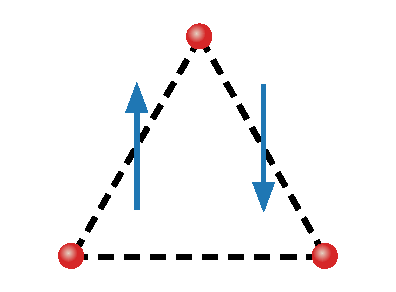
\includegraphics[width=3.0 in]{./figures/3-point-triangle.pdf}}
  \subfloat[]{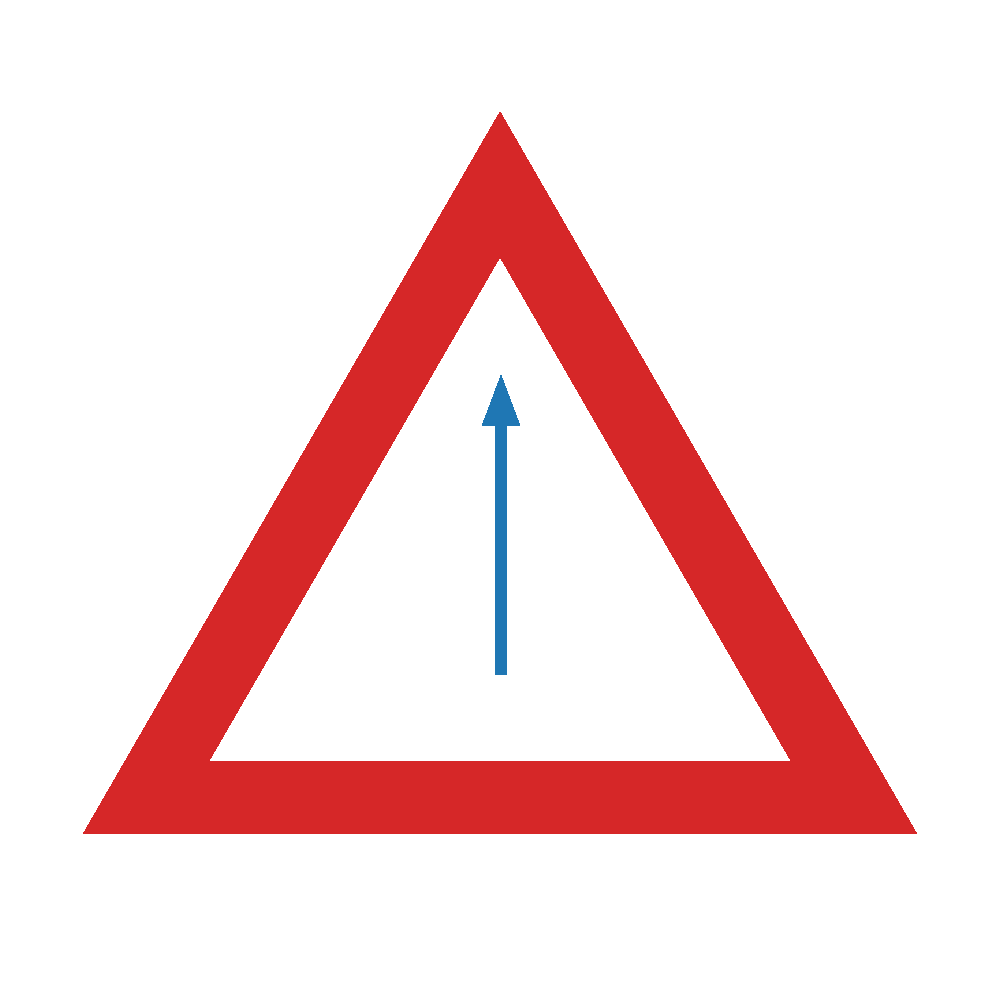
\includegraphics[width=2.4 in]{./figures/hollow-triangle-constant-vector-potential.pdf}}
  \caption{Schematics of two triangle structures proposed in this work. (a) Three-site Kitaev triangle with bond-dependent Peierls phases. (b) Hollow triangular island with a uniform vector potential.}
  \label{fig:triangles}
\end{figure}


In this section we present an exactly solvable minimal model with three sites forming a ``Kitaev triangle" that can host MZM at different pairs of vertices controlled by Peierls phases on the edges. The Bogoliubov-de Gennes (BdG) Hamiltonian includes complex hopping and $p$-wave pairing between three spinless fermions forming an equilateral triangle [Fig.~\ref{fig:triangles} (a)]:
\begin{equation}\label{eq:HBdG}
  \ham = \sum_{\langle j l \rangle} (-te^{i\phi_{jl}}\cc_{j} c_l + \de e^{i\theta_{jl}} c_{j} c_l + {\rm h.c.}) - \sum_{j} \mu \cc_j c_j,
\end{equation}
where $t$ is the hopping amplitude, $\de$ is the amplitude of the (2D) $p$-wave pairing, $\mu$ is the chemical potential, $\theta_{jl}$ is the polar angle of $\mathbf r_{jl} = \mathbf r_l - \mathbf r_j$ (the $x$ axis is chosen to be along $\mathbf r_{12}$), consistent with $\{c^\dag_l, c^\dag_j\} = 0$. $\phi_{jl}$ is the Peierls phase due to a bond-dependent vector potential $\mathbf A$ to be specified below (the nearest neighbor distance $a$ is chosen to be the length unit hereinbelow):
\begin{eqnarray}
\phi_{jl} = \dfrac{e}{\hbar} \int_{\mathbf r_j}^{\mathbf r_{l}} \vec{A} \cdot d\vec{l} = -\phi_{lj}
\end{eqnarray}
where $e>0$ is the absolute value of the electron charge. Below we use the natural units $e=\hbar=1$. To get the conditions for having MZM in this model we rewrite $\mathcal{H}$ in the Majorana fermion basis $a_{j} = c_j + c^\dag_j$, $b_j = \frac{1}{i}(c_j - c^\dag_j)$:
\begin{align}\label{eq:H3M}
    \ham =  -\dfrac{i}{2} \sum_{\langle j l \rangle} \Big[&\left(t\sin\phi_{jl}-\de\sin\theta_{jl}\right) a_j a_l \\\nonumber
  +&\left(t\sin\phi_{jl}+\de\sin\theta_{jl}\right) b_j b_l  \\\nonumber
  +&\left(t\cos\phi_{jl} - \de\cos\theta_{jl}\right) a_j b_l  \\\nonumber
  -&\left(t\cos\phi_{jl}+\de\cos\theta_{jl}\right) b_j a_l\Big]  -\dfrac{i\mu}{2} \sum_j  a_j b_j
\end{align}
For concreteness we consider the Kitaev limit $t=\de$, $\mu=0$, and choose $\phi_{12} = 0$ so that sites 1 and 2 alone form a minimal Kitaev chain with $\mathcal{H}_{12} = itb_1a_2$ and hosting MZM $a_1$ and $b_2$. In order for the MZM to persist in the presence of site 3, one can choose $\phi_{23}$ and $\phi_{31}$ so that all terms involving these Majorana operators cancel out. For example, consider the $2-3$ bond, for which $\theta_{23} = 2\pi/3$, we require
\begin{eqnarray}
    \sin\phi_{23} + \sin\frac{2\pi}{3} =\cos\phi_{23} + \cos\frac{2\pi}{3} = 0
\end{eqnarray}
which means $\phi_{23} = -\pi/3$. Similarly one can find $\phi_{31} =-\phi_{13} = -\pi/3$. The three Peierls phases can be realized by the following staggered vector potential
\begin{equation}\label{eq:Astep}
  \vec{A} =\left[1-2\Theta(x)\right]\frac{2 \pi}{3\sqrt{3}} \hat{y}
\end{equation}
where $\Theta(x)$ is the Heavisde step function. In fact, using a uniform $\vec{A} =\frac{2 \pi}{3\sqrt{3}} \hat{y}$, which corresponds to $\phi_{23} = -\pi/3 = -\phi_{31}$ also works, since the existence of $a_1$ is unaffected by $\phi_{23}$. However, in this case the counterpart of $b_2$ is not localized on a single site. For the same reason, the above condition for MZM localized at triangle corners can be generalized to Kitaev chains forming a triangular loop, as well as to finite-size triangles of 2D spinless $p$-wave superconductors in the Kitaev limit, as the existence of $a_1$ and $b_2$ are only dictated by the vector potential near the corresponding corners. It should be noted that in the latter case, 1D Majorana edge states will arise when the triangle becomes larger, and effectively diminish the gap that protects the corner MZM.  On the other hand, for the longer Kitaev chain, due to the potential practical difficulty of controlling further-neighbor hopping and pairing amplitudes, it is better to resort to the approach of controlling the individual topological phases of the three edges which will be detailed in the next section.

We next show that the minimal Kitaev triangle suffices to demonstrate braiding of MZM. To this end we consider a closed parameter path linearly interpolating between the following sets of values of $\phi_{jl}$:
\begin{eqnarray}
    (\phi_{12},\phi_{23},\phi_{31}) &=& \left(0,-\frac{\pi}{3},-\frac{\pi}{3}\right ) \equiv \bm \phi_1 \\\nonumber
    &\rightarrow& \left(-\frac{\pi}{3},-\frac{\pi}{3},0 \right) \equiv \bm \phi_2 \\\nonumber
    &\rightarrow& \left(-\frac{\pi}{3},0,-\frac{\pi}{3} \right) \equiv \bm \phi_3 \\\nonumber
    &\rightarrow& \bm \phi_1
\end{eqnarray}
It is straightforward to show that at $\bm \phi_{2}$ and $\bm \phi_3$ there are MZM located at sites $3,1$ and $2,3$, respectively. Therefore the two original MZM at sites $1,2$ should switch their positions at the end of the adiabatic evolution.

\begin{figure}[!ht]
	\centering
  \hspace{-27pt}
  \subfloat[]{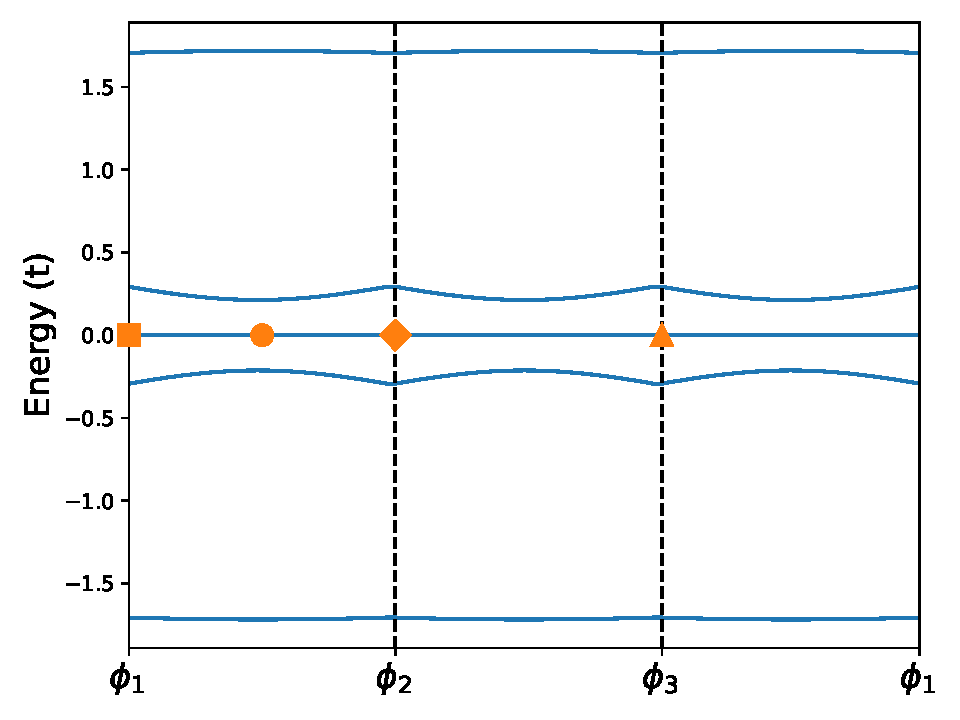
\includegraphics[width=3.3 in]{./figures/3eigval.pdf}}\\
  \subfloat[]{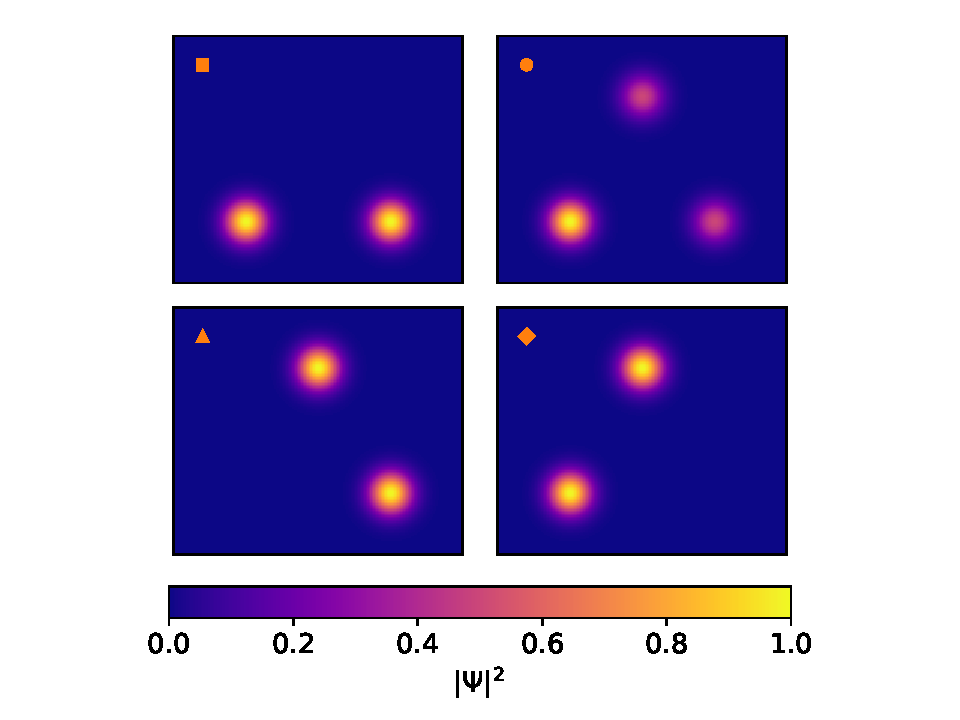
\includegraphics[width=4.2 in]{./figures/3eigvec.pdf}}
	\caption{(a) Evolution of the eigenvalues of the 3-site Kitaev triangle along the closed parameter path for $\phi$ on the three edges. (b) MZM wavefunctions at different points of the parameter path. Clockwise from the upper left panel: $\bm \phi_1 \rightarrow \frac{1}{2}(\bm \phi_1 + \bm \phi_2)\rightarrow \bm \phi_2\rightarrow \bm \phi_3$.}
	\label{fig:3eig}
\end{figure}

Indeed, Fig.~\ref{fig:3eig} shows that the MZM stays at zero energy throughout the parameter path that interchanges their positions. To show that such an operation indeed realizes braiding, we explicitly calculated the many-body Berry phase of the evolution \cite{supp,aliceaNonAbelianStatisticsTopological2011,liManipulatingMajoranaZero2016} and found the two degenerate many-body ground states acquire a $\frac{\pi}{2}$ difference in their Berry phases as expected \cite{aliceaNonAbelianStatisticsTopological2011}. Compared to the minimum T-junction model with four sites \cite{aliceaNonAbelianStatisticsTopological2011}, our Kitaev triangle model only requires three sites to achieve braiding between two MZM, and is potentially also easier to engineer experimentally. In the next section we will show that a more mesoscopic hollow-triangle structure can achieve similar results and may be preferred in other materials platforms.


\section{Hollow Triangles}

For systems with less fine-tuned Hamiltonians than the minimal model in the previous section, it is more instructive to search for MZM based on topological arguments. In this section we show that MZM generally appear at the corners of a hollow triangle, which can be approximated by joining three finite-width chains or ribbons whose bulk topology is individually tuned by the same uniform vector potential.

To this end, we first show that topological phase transitions can be induced by a vector potential in a spinless $p$-wave superconductor ribbon. In comparison with similar previous proposals that mostly focused on vector potentials or supercurrents flowing along the chain \cite{romitoManipulatingMajoranaFermions2012, takasanSupercurrentinducedTopologicalPhase2022}, we consider in particular the tunability by varying the direction of the vector potential relative to the length direction of the ribbon, which will become instrumental in a triangular structure.

Consider Eq.~\eqref{eq:HBdG} on a triangular lattice defined by unit-length lattice vectors $(\mathbf a_1, \mathbf a_2) = (\hat{x}, \frac{1}{2}\hat{x} + \frac{\sqrt{3}}{2}\hat{y})$ with $W$ unit cells along $\mathbf a_2$ but infinite unit cells along $\mathbf a_1$, and assume the Peierls phases are due to a uniform vector potential $\mathbf A$ so that $\phi_{jl} = \mathbf A\cdot \mathbf r_{jl}$. We also introduce $\mathbf a_3 \equiv -\mathbf a_1 + \mathbf a_2$ for later convenience. The Hamiltonian is periodic along $x$ and can be Fourier transformed through $\cc_{m,n} = \dfrac{1}{\sqrt{N}} \sum_{k} \cc_{k,n} e^{-i km}$, where $m,n$ label the lattice sites as $\mathbf r_{m,n} = m\mathbf a_1 + n \mathbf a_2$. The resulting momentum space Hamiltonian can be written as the following block form up to a constant
\begin{eqnarray}\label{eq:Hribbon}
      \ham &=& \dfrac{1}{2} \sum_k \Psi_k^\dagger \left(
    \begin{matrix}
      h_t(k) & h_\Delta(k) \\
      h_\Delta^\dagger(k) & -h_t^*(-k)
    \end{matrix} \right)
    \Psi_k \\\nonumber
&\equiv&\dfrac{1}{2} \sum_k \Psi_k^\dagger H(k)
    \Psi_k
\end{eqnarray}
where $\Psi_k \equiv (c_{k,1},\dots, c_{k,W},c^\dag_{-k,1},\dots c_{-k,W}^\dag)^T$. $h_t(k)$ is a $W\times W$ Hermitian tridiagonal matrix with $(h_t)_{n,n} = -2t\cos(k+\mathbf A\cdot \mathbf a_1) - \mu$ and $(h_t)_{n,n+1} = -t\left( e^{i(-k+\mathbf A\cdot \mathbf a_3)}  + e^{i\mathbf A \cdot \mathbf a_2}\right)$. $h_\Delta(k)$ is a $W\times W$ tridiagonal matrix with $(h_\Delta)_{n,n} = -2i\de \sin k $ and $(h_\Delta)_{n,n\pm 1} = \mp \de\left[ e^{-i(\pm k + \frac{2\pi}{3})} + e^{-i\frac{\pi}{3}} \right]$.

By transforming Eq.~\eqref{eq:Hribbon} to the Majorana basis using the unitary transformation:
\begin{eqnarray}
    U\equiv \dfrac{1}{\sqrt{2}} \left(
  \begin{matrix}
    1 & 1 \\
    -i & i
  \end{matrix} \right) \otimes \mathbb{I}
\end{eqnarray}
where $\mathbb{I}$ is a ${W\times W}$ identity matrix, and defining $A_k\equiv -iU H(k) U^\dag$, not to be confused with the vector potential, one can calculate the Majorana number \cite{kitaevUnpairedMajoranaFermions2001} $\mathcal{M}$ of the 1D ribbon as \cite{liTopologicalSuperconductivityInduced2014}
\begin{eqnarray}
\mathcal{M} = {\rm sgn}\left[{{\rm Pf}(A_{k=0}) {\rm Pf}(A_{k=\pi})}\right]
\end{eqnarray}
where $\text{Pf}$ stands for the Pfaffian of a skew-symmetric matrix \cite{kitaevUnpairedMajoranaFermions2001}. When $\mathcal{M} = -1$, the 1D system is in a nontrivial topological phase with MZM appearing at open ends of semi-infinite ribbons, and otherwise for $\mathcal{M} = 1$.

\begin{figure}[!ht]
  \hspace{12pt}
  \subfloat[]{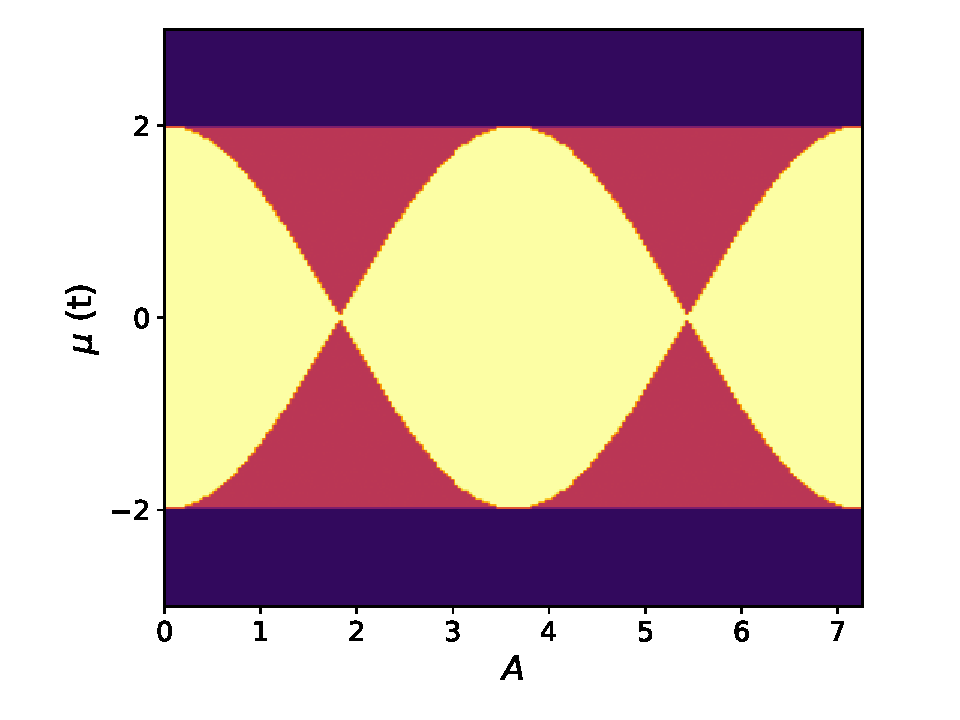
\includegraphics[width=0.532\textwidth]{./figures/topological-phase-diagram-1pi6-n-1.pdf}} \\
  \vspace{-15pt}
  \subfloat[]{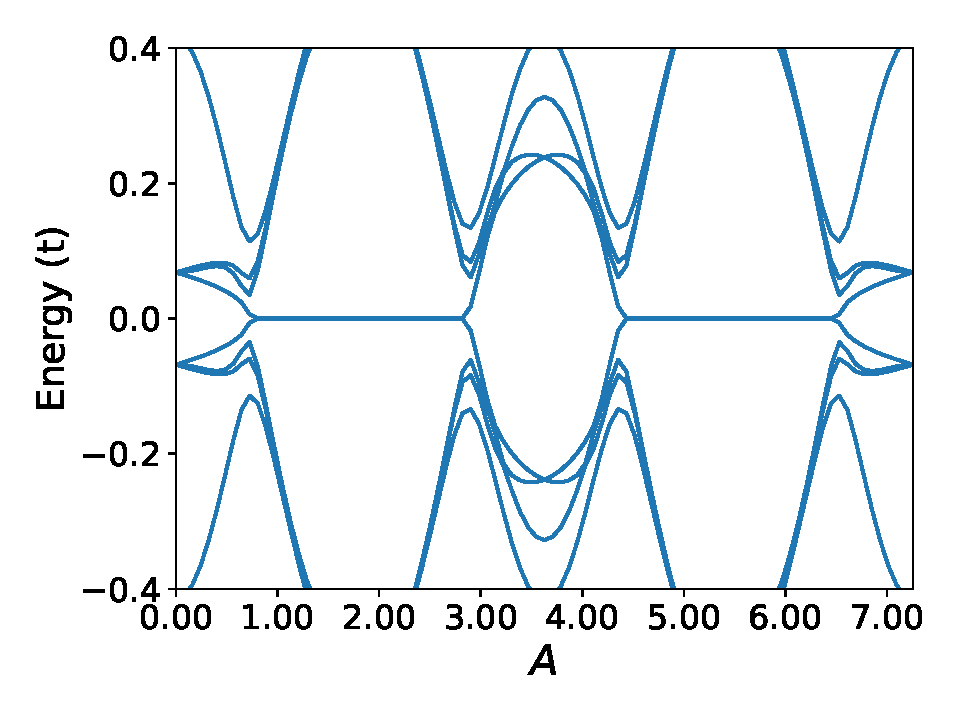
\includegraphics[width=0.50\textwidth]{./figures/spectral-flow-nr-50-w-1-mu-1_6.pdf}}
\caption{(a) Topological phase diagram for a $W=1$ triangular chain with the Hamiltonian Eq.~\eqref{eq:Hribbon} obtained by superimposing the $\mathcal{M}(A, \mu)$ plots of 1D chains with $\mathbf A = A\hat{y}$ and $\mathbf A = A(\frac{\sqrt{3}}{2}\hat{x}+\frac{1}{2}\hat{y})$. Color scheme: white---$\mathcal{M}=1$, dark blue---$\mathcal{M}=-1$, light blue---$\mathcal{M}=0$ (b) Near-gap BdG eigen-energies vs $A$ for a finite triangle with edge length $L = 50$, $W=1$, and $\mu=1.6$.}
  \label{fig: pd}
\end{figure}

In Fig.~\ref{fig: pd} (a) we show the topological phase diagrams for a 1D ribbon with width $W=1$, $\mathbf A = A\hat{y}$ and $\mathbf A = A(\frac{\sqrt{3}}{2}\hat{x}+\frac{1}{2}\hat{y})$ superimposed (see below). We found that the vector potential component normal to the ribbon length direction has no effect on the Majorana number, nor does the sign of its component along the ribbon length direction. However, topological phase transitions can be induced by varying the size of the vector potential component along the ribbon, consistent with previous results \cite{romitoManipulatingMajoranaFermions2012, takasanSupercurrentinducedTopologicalPhase2022}. These properties motivate us to consider the structure of a hollow triangle formed by three finite-width ribbons subject to a uniform vector potential $\mathbf A = A\hat{y}$ as illustrated in Fig.~\ref{fig:triangles} (b). The light blue color on the phase diagram Fig.~\ref{fig: pd} (a) therefore means that the bottom edge and the two upper edges of the hollow triangle have different $\mathcal{M}$, which should give rise to MZM localized at the two bottom corners if the triangle is large enough so that bulk-edge correspondence holds, and gap closing does not occur at other places along its edges.

To show that corner MZM indeed appear when the conditions given by the phase diagram Fig.~\ref{fig: pd} (a) are met, we directly diagonalize the BdG Hamiltonian of a finite hollow triangle with edge length $L=50$ and width $W=1$. Fig.~\ref{fig: pd} (b) shows the spectral flow (BdG eigen-energies evolving with increasing vector potential $A$) close to zero energy at chemical potential $\mu=1.6$. Indeed, zero-energy modes appear in the regions of $\mu$ and $A$ consistent with the phase diagram (except when the bulk band gap is too small; see \cite{supp} for some examples.). Hollow triangles with larger larger $W$ also have qualitatively similar behavior, although the phase diagrams are more complex \cite{supp}. The eigenfunctions for the zero-energy modes at $A=2.75$ and $\mu=1.6$ in Fig.~\ref{fig: rotation} (b) also confirm their spatial localization at the bottom corners of the triangle.

\begin{figure*}[!ht]
  \subfloat[]{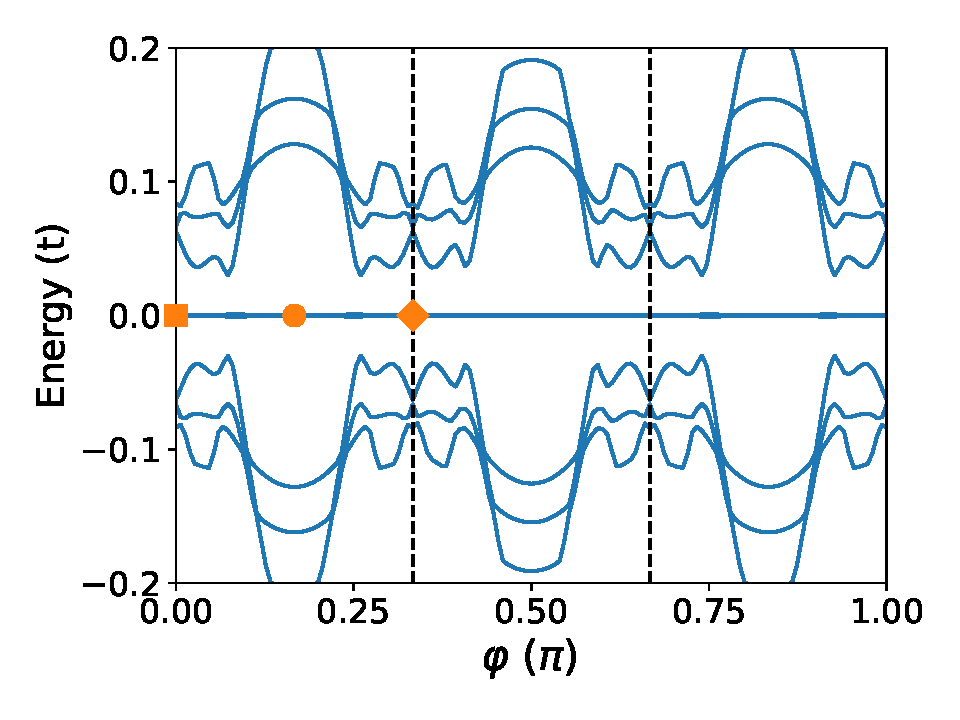
\includegraphics[height=150pt]{./figures/spectral-flow-rotation-constant-vector-nr-50-w-1-mu-1_6.pdf}} \\
  \subfloat[]{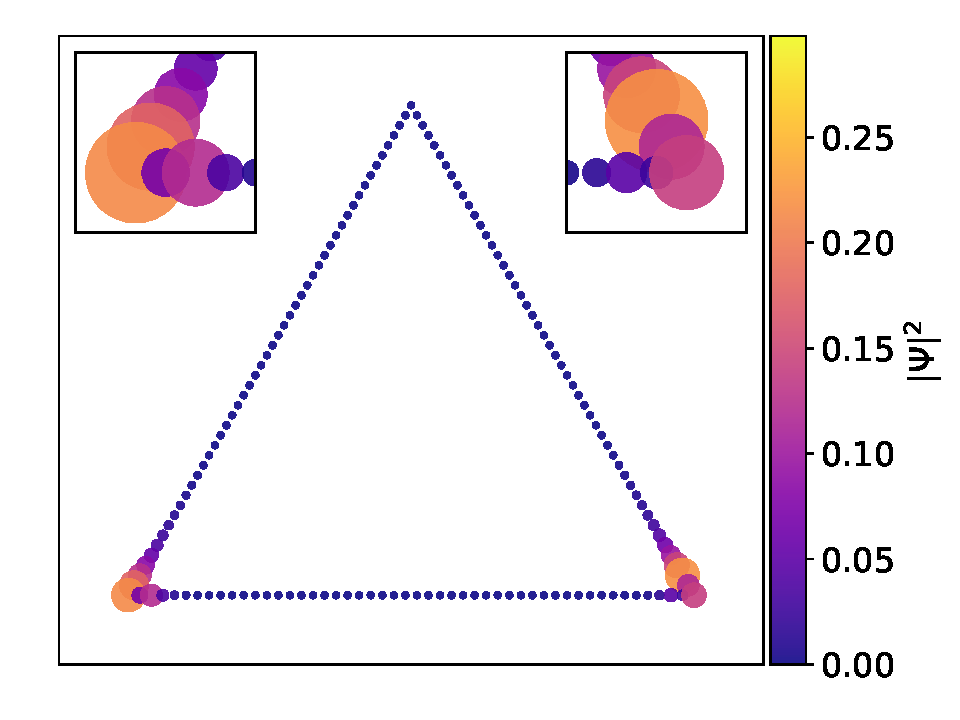
\includegraphics[height=125pt]{./figures/GS-T-Square.pdf}}
  \hspace{-20pt}
  \subfloat[]{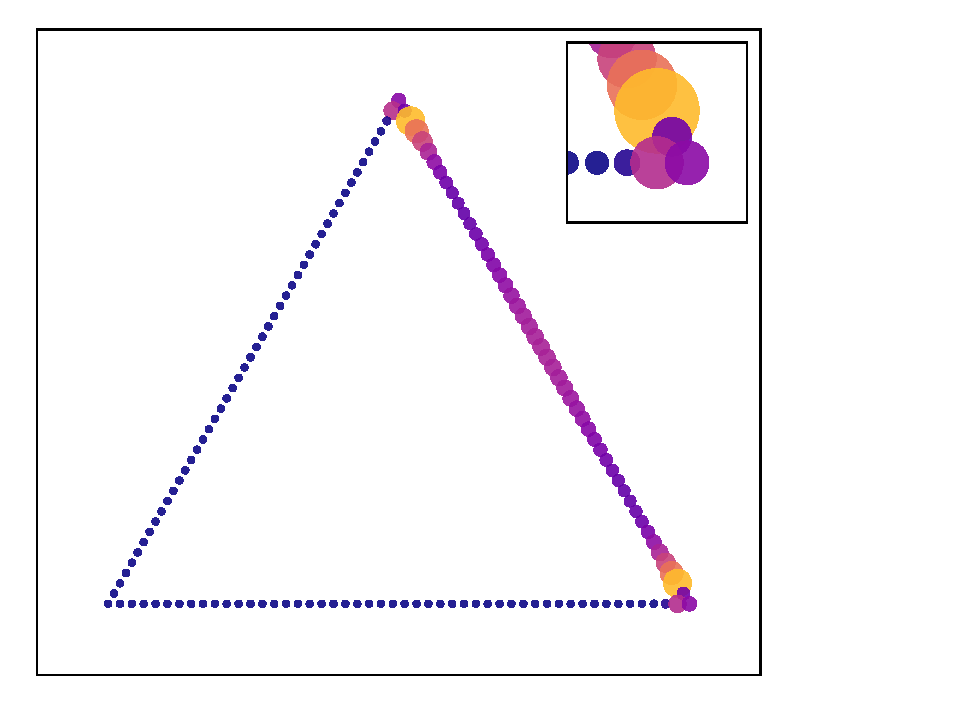
\includegraphics[height=125pt]{./figures/GS-T-Circle.pdf}}
  \hspace{-24pt}
  \subfloat[]{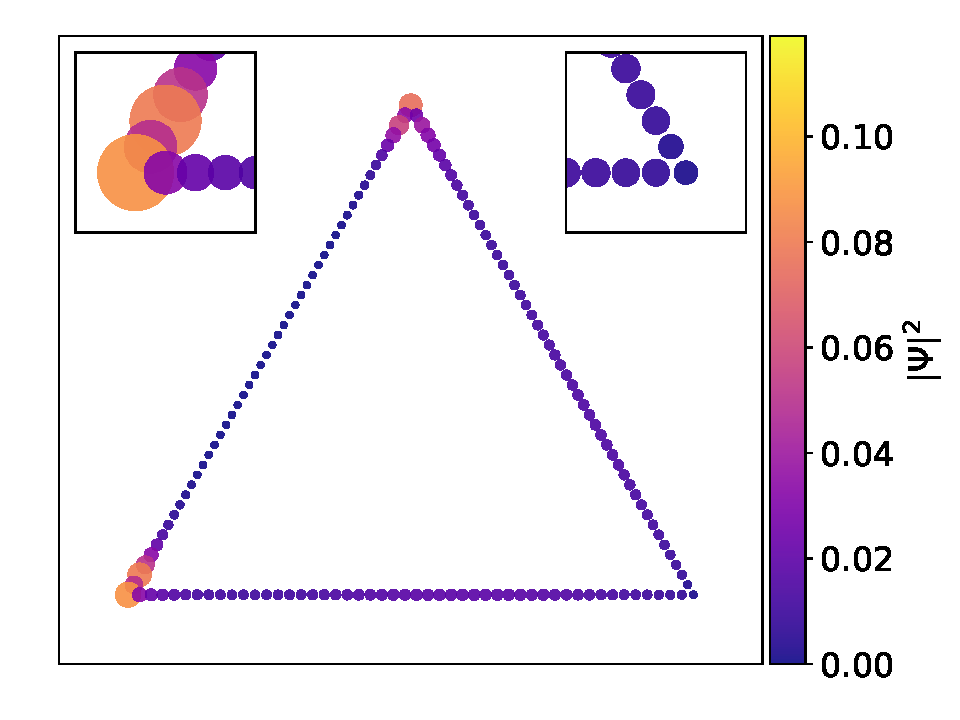
\includegraphics[height=127pt]{./figures/GS-T-Diamond.pdf}}
  \caption{(a) Spectral flow of a hollow triangle with $W=1$, $L=50$, $\mu=1.6$, and $A=2.75$ with increasing rotation angle $\varphi$, defined through $\mathbf A = A(-\sin\varphi \hat{x} + \cos\varphi \hat{y})$. (b-d) BdG eigenfunction $|\Psi|^2$ summed over the two zero modes at $\varphi = 0, \frac{\pi}{6}$, and $\frac{\pi}{3}$, respectively.}
  \label{fig: rotation}
\end{figure*}

We finally show that rotating the uniform vector potential in-plane can manipulate the positions of the MZM without hybridizing them with bulk states for certain ranges of $\mu$ and $A$. Fig.~\ref{fig: rotation} (a) plots the spectral flow versus the in-plane azimuthal angle of $\mathbf A$, which clearly shows that the zero-energy modes persist throughout the rotation and the bulk gap never closes. Figs.~\ref{fig: rotation} (b-d) plot the BdG wavefunctions of the MZM at special values of $\varphi$. One can see that the two MZM appear to cycle through the three vertices by following the rotation of $\mathbf A$. The robustness of the MZM therefore requires the condition of two edges being in a different topological phase from the third one to be satisfied throughout the rotation. Such a criterion combined with the individual phase diagrams of the edges can help isolate the desired parameter regions of $\mu$ and $A$. We also note that the positions of the MZM do not interchange after $\varphi$ increases from 0 to $\pi$, different from the situation of the minimal Kitaev triangle in Fig.~\ref{fig:3eig}. The reason is that the MZM in the latter case are not due to bulk-boundary correspondence [the values of $A = \frac{2\pi}{3\sqrt{3}}$ and $\mu=0$ are a critical point in the phase diagram Fig.~\ref{fig: pd} (a)]. While the positions of the MZM at special points along the parameter path in the hollow triangle case have to be additionally constrained by the bulk topological phases of the three edges, that for the Kitaev triangle have more flexibility and are also protected by the finite size of the system.



\begin{figure}[!ht]
  \hspace{28pt}
  \subfloat[]{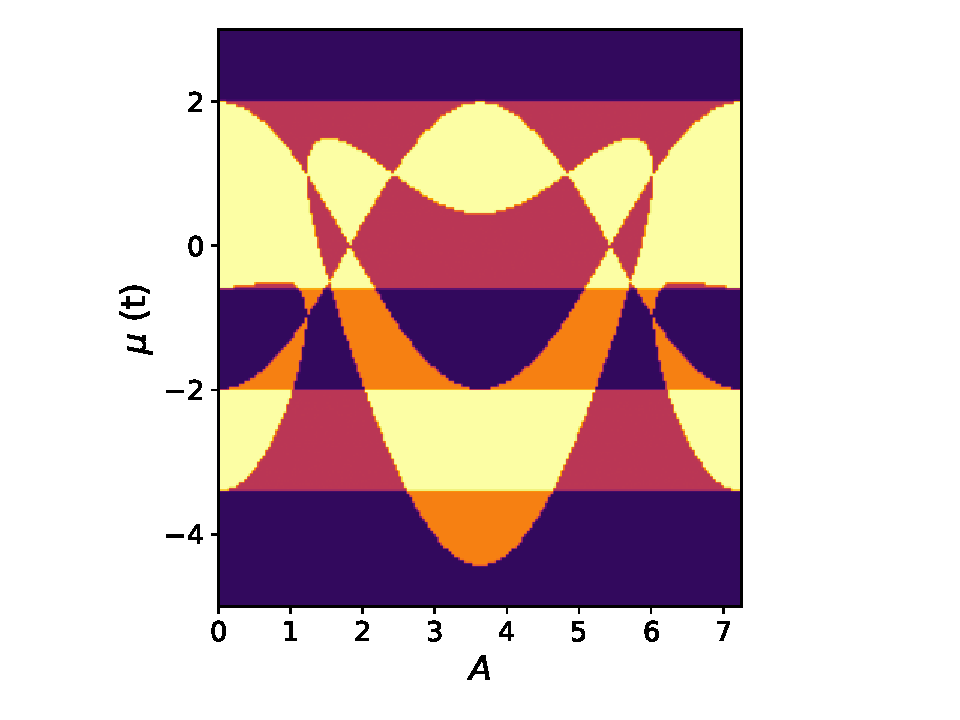
\includegraphics[width=0.50\textwidth]{./figures/supp/topological-phase-diagram-1pi6-n-3.pdf}}
  \hspace{-40pt}
  \subfloat[]{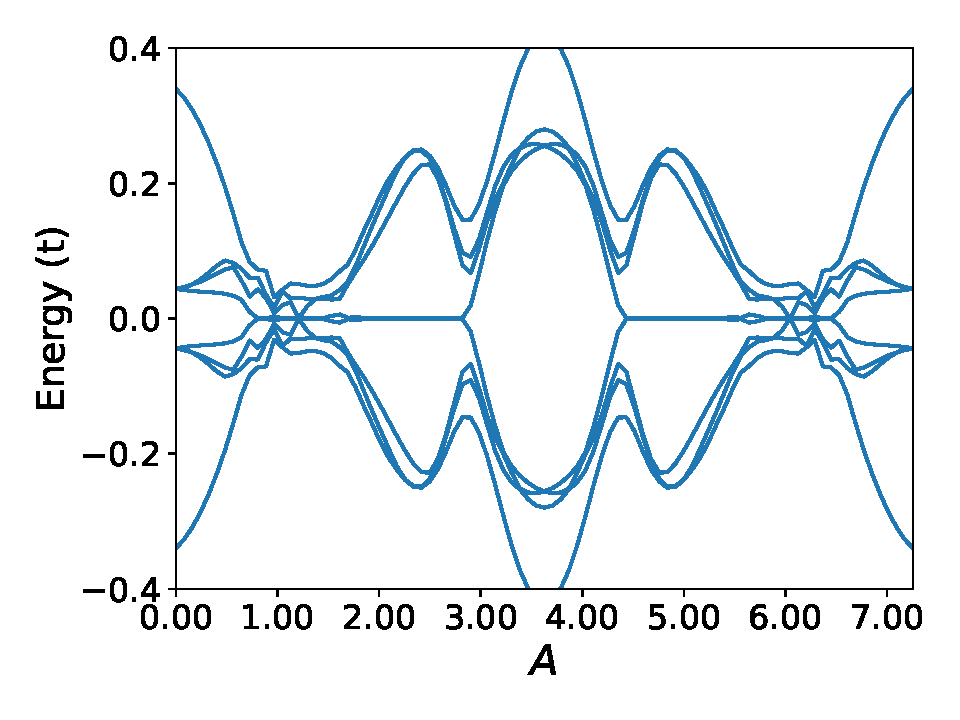
\includegraphics[width=0.50\textwidth]{./figures/supp/spectral-flow-nr-50-w-3-mu-1_6.pdf}} \\
  \hspace{70pt}
  \subfloat[]{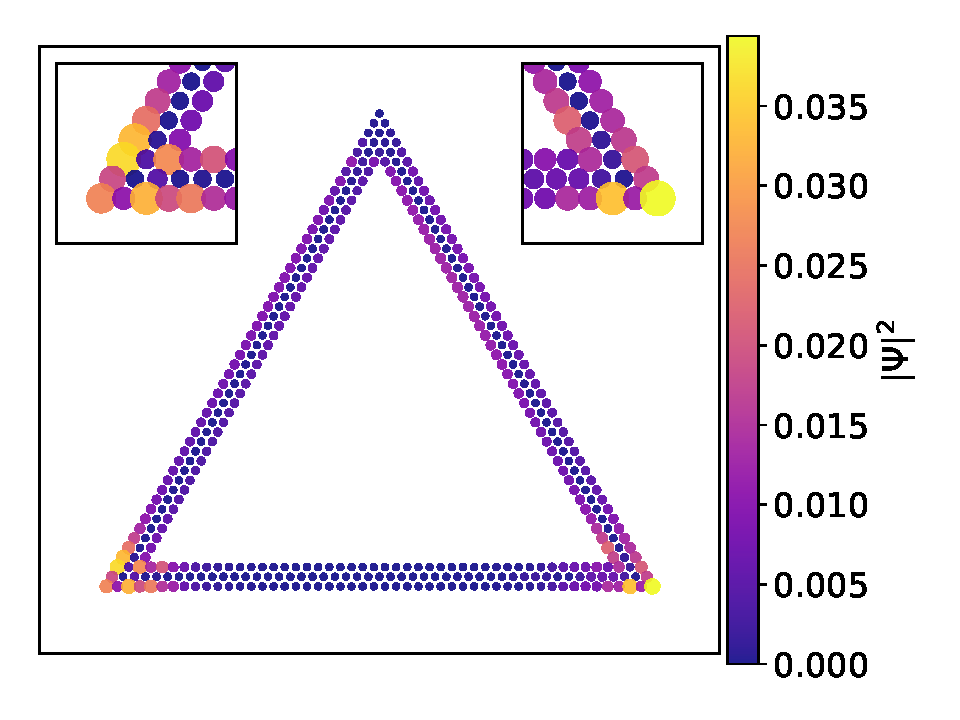
\includegraphics[width=0.50\textwidth]{./figures/supp/GS-A-2_74-nr-50-w-3-mu-1_6.pdf}}
  \caption{(a) Topological phase diagram for a $W=3$ hollow triangle obtained by overlapping the $\mathcal{M}(A, \mu)$ plots of 1D chains with $\mathbf A = A\hat{y}$ and $\mathbf A = A(\frac{\sqrt{      3}}{2}\hat{x}+\frac{1}{2}\hat{y})$. Color scheme: white---$\mathcal{M}=1$, dark blue---$\mathcal{M}=-1$, light blue---$\mathcal{M}=0$ (b) Near-gap BdG eigen-energies vs $A$ for a finite triangle with edge length $L=50$, $W=3$, and $\mu=1.6$. (c) BdG eigenfunction $|\Psi|^2$ summed over the two zero modes at $A=2.4709$.}
  \label{fig: supp pd}
\end{figure}

A model that is closer to a realistic hollow triangular island is the finite-width triangular chain or ribbon. An example, illustrated in Figure \ref{fig: supp pd} (c), has its edge length $L=50$ and width $W=3$. The phase diagram Fig.~\ref{fig: supp pd} (a) is created in a similar way as that in Fig. \ref{fig: pd} (a), assuming a constant vector potential and infinitely long $W=3$ ribbons. The spectral flow for the actual triangle with $\mu = 1.6$ in Fig.~\ref{fig: supp pd} (b) shows MZM in the parameter regions in agreement with the phase diagram. Fig.~\ref{fig: supp pd} (c) plots the MZM wavefunction for $A=2.7409$ and $\mu=1.6$ that are indeed well localized at the bottom corners.

\begin{figure}[!ht]
  \hspace{-20pt}
  \subfloat[]{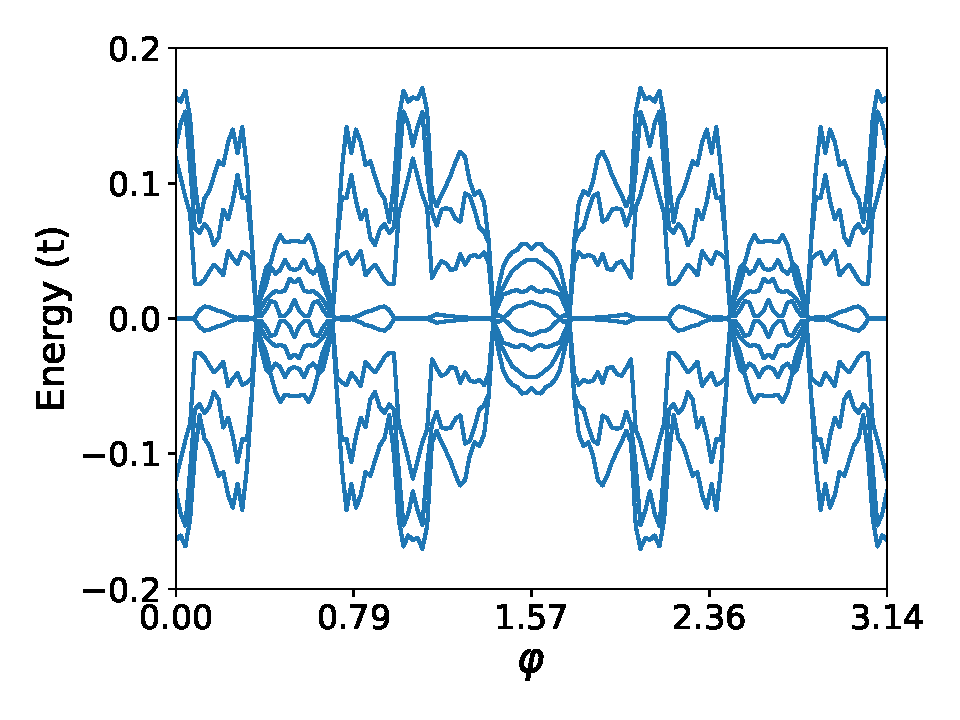
\includegraphics[width=0.5\textwidth]{./figures/supp/spectral-flow-w-3.pdf}}\\
  \subfloat[]{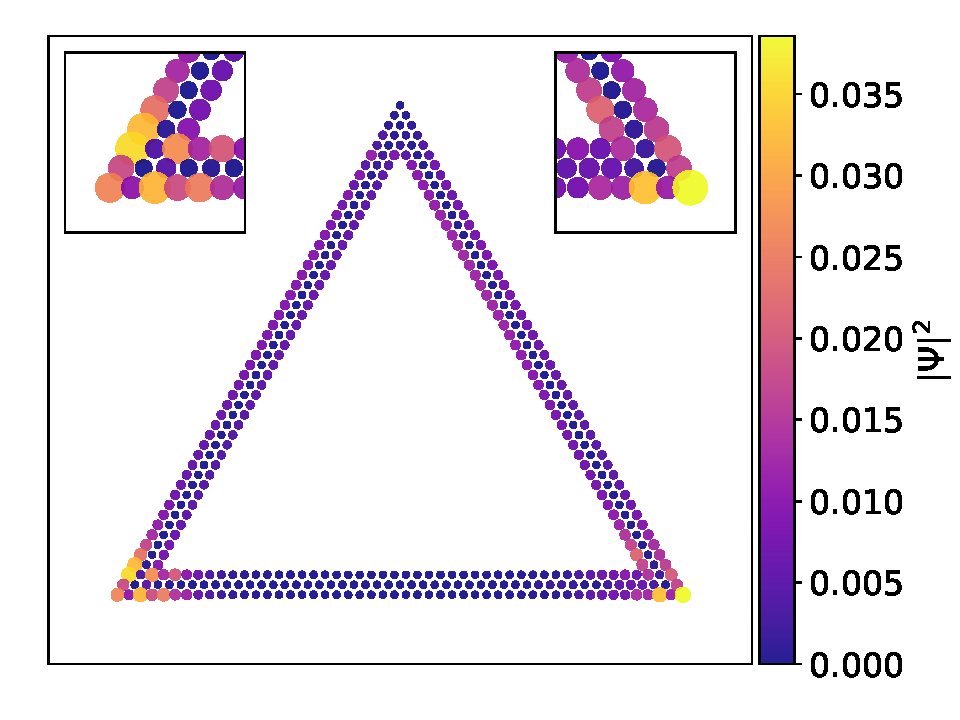
\includegraphics[width=0.4\textwidth]{./figures/supp/GS-T-Square-w-3.pdf}}
  %\subfloat[]{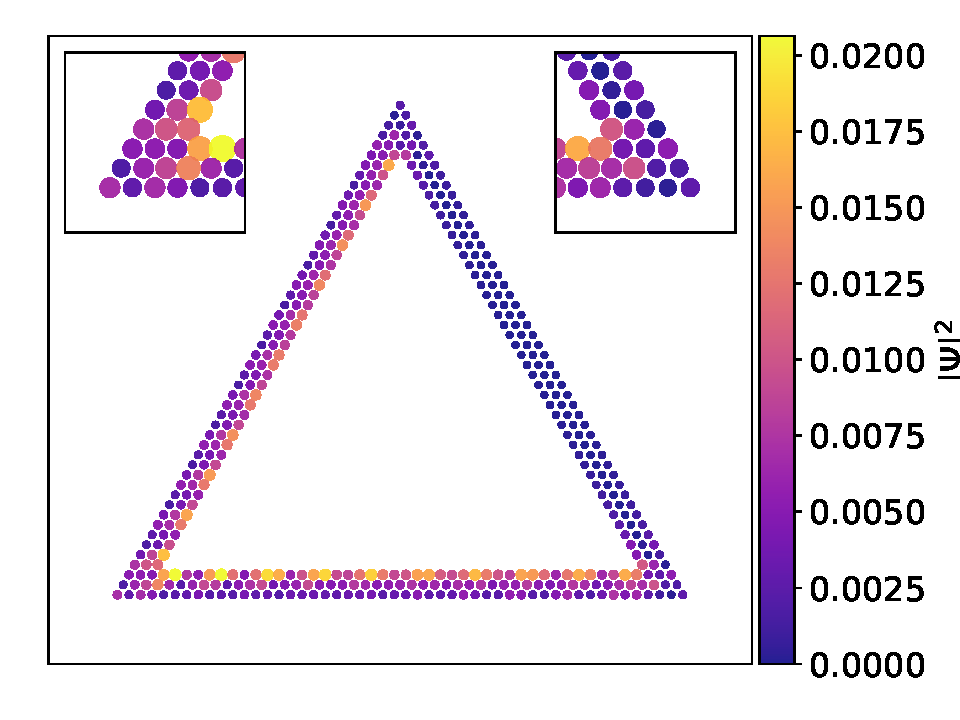
\includegraphics[width=0.4\textwidth]{./figures/supp/GS-T-Circle-w-3.pdf}}
  \subfloat[]{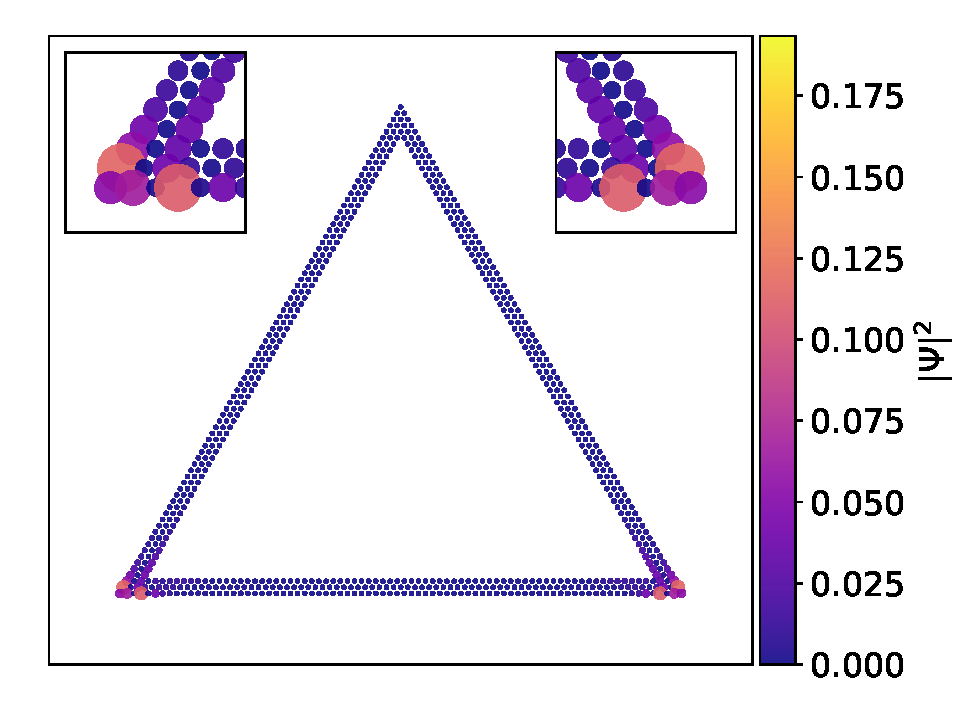
\includegraphics[width=0.4\textwidth]{./figures/supp/GS-T-Diamond-w-3.pdf}}
  \caption{(a) Spectral flow of a hollow triangle with $W=3$, $L=50$, $\mu=1.6$, and $A=2.75$ with increasing rotation angle $\varphi$, defined through $\mathbf A = A(-\sin\varphi \hat{x} + \cos\varphi \hat{y})$. (b-c) BdG eigenfunction $|\Psi|^2$ summed over the two zero modes at $\varphi = 0$ and $\frac{\pi}{3}$, respectively.}
  \label{fig: supp rotation}
\end{figure}

We next rotate the uniform vector potential to examine how the MZM move on a hollow triangle. Figure~\ref{fig: supp rotation} shows the spectral flow and eigenfunctions as we rotate $\varphi=0$ to $\varphi=\pi$ counterclockwisely. The two MZM cycle through the three vertices in a similar manner as that in Fig.~4 of the main text (only the MZM wavefunctions at $\varphi = 0$ and $\frac{\pi}{3}$ are plotted as representatives of the $\varphi = n\pi/3$ cases). Note that the spectral flow has 3-fold rotation symmetry but not 6-fold, since increasing $\varphi$ by $\frac{2\pi}{3}$ is equivalent to rotating the coordinate system clockwisely by $\frac{2\pi}{3}$. In contrast, rotating the vector potential by $\frac{\pi}{3}$, if without an additional sign change of the $p$-wave pairing potential, is not an exact symmetry of the finite triangle. Also we did not try to scrutinize the phase diagram to find a parameter path in which the bulk gap does not close, as in the $W=1$ case in the main text. Here we just point out that identifying a system-specific parameter path for adiabatic manipulation of MZM is in principle always possible, especially if one is allowed to have more knobs other than $\varphi$ in real structures, such as tuning the chemical potential of individual edges or the size of the vector potential, etc.

\section{Braiding MZM in a small network of triangles}

\begin{figure}[!ht]
  \hspace{-30pt}
  \subfloat[]{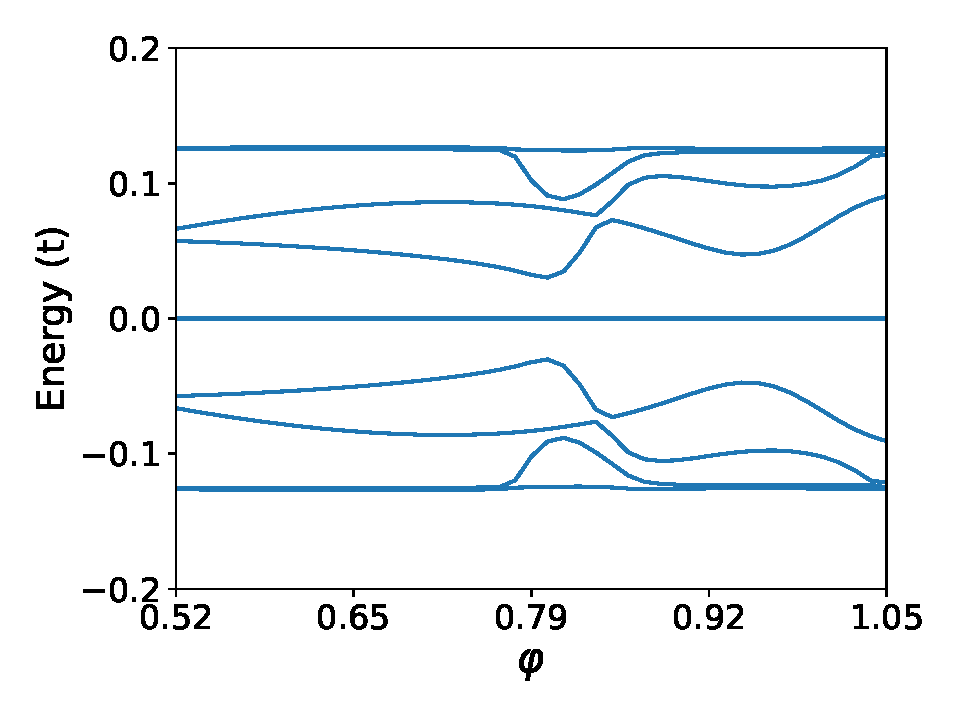
\includegraphics[width=0.4\textwidth]{./figures/supp/spectral-flow-braiding.pdf}} \\
  \vspace{-10pt}
  \subfloat[]{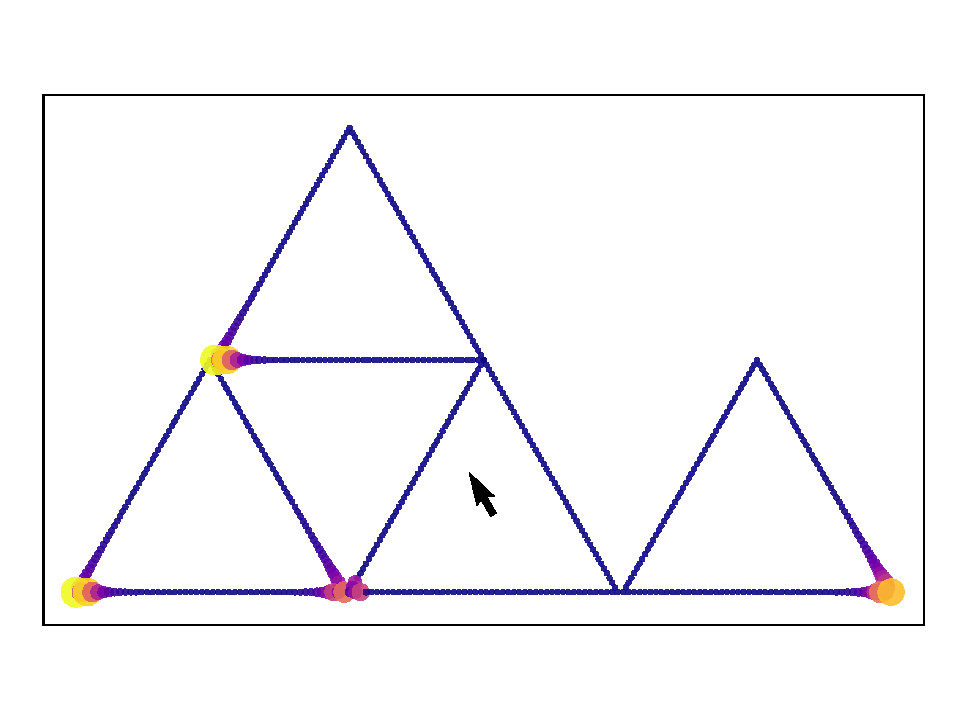
\includegraphics[width=0.30\textwidth]{./figures/supp/GS-T-0_5236.pdf}}
  \subfloat[]{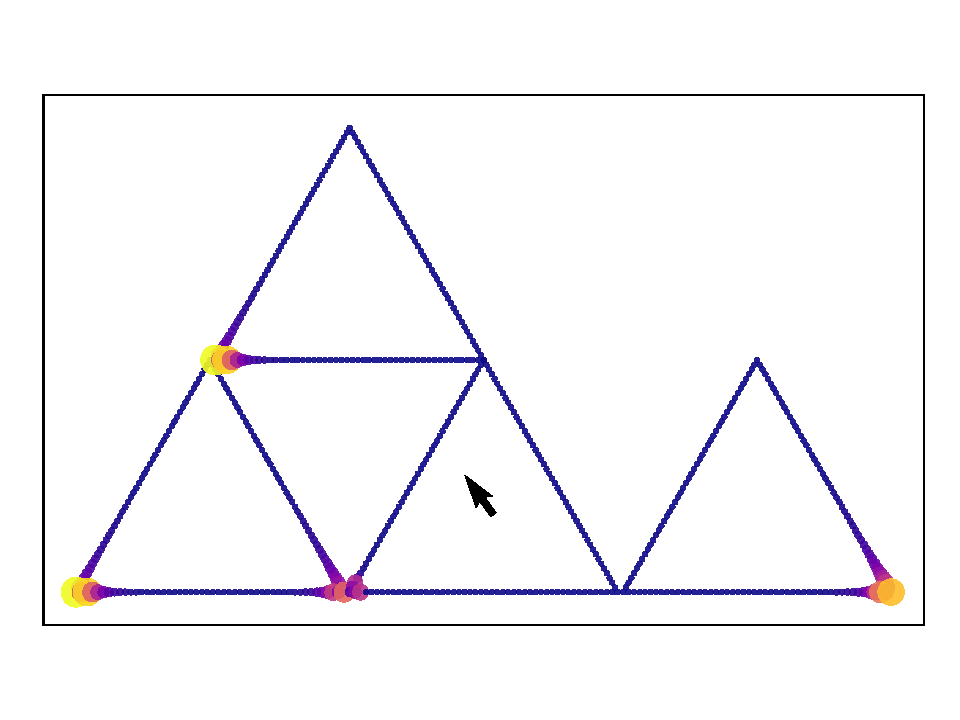
\includegraphics[width=0.30\textwidth]{./figures/supp/GS-T-0_6283.pdf}}
  \subfloat[]{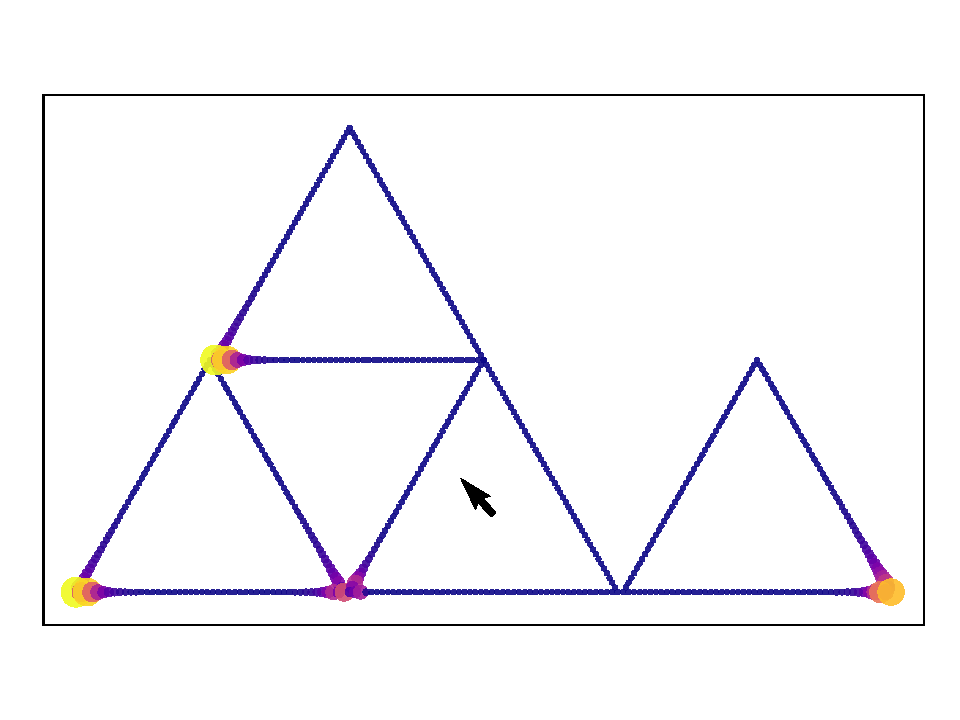
\includegraphics[width=0.30\textwidth]{./figures/supp/GS-T-0_7330.pdf}} \\
  \subfloat[]{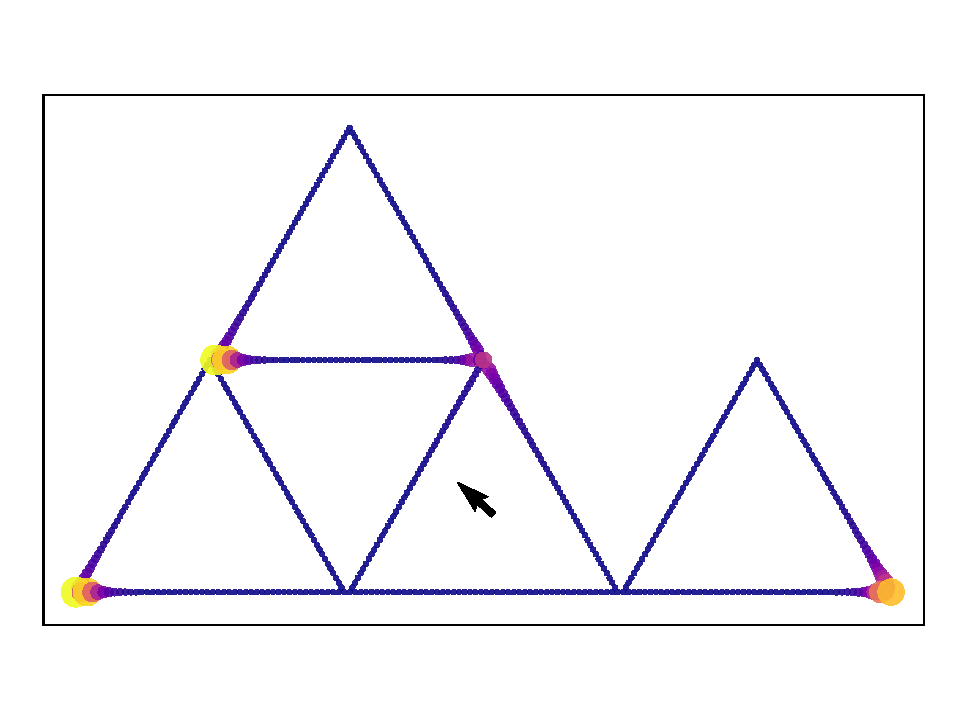
\includegraphics[width=0.30\textwidth]{./figures/supp/GS-T-0_8378.pdf}}
  \vspace{-10pt}
  \subfloat[]{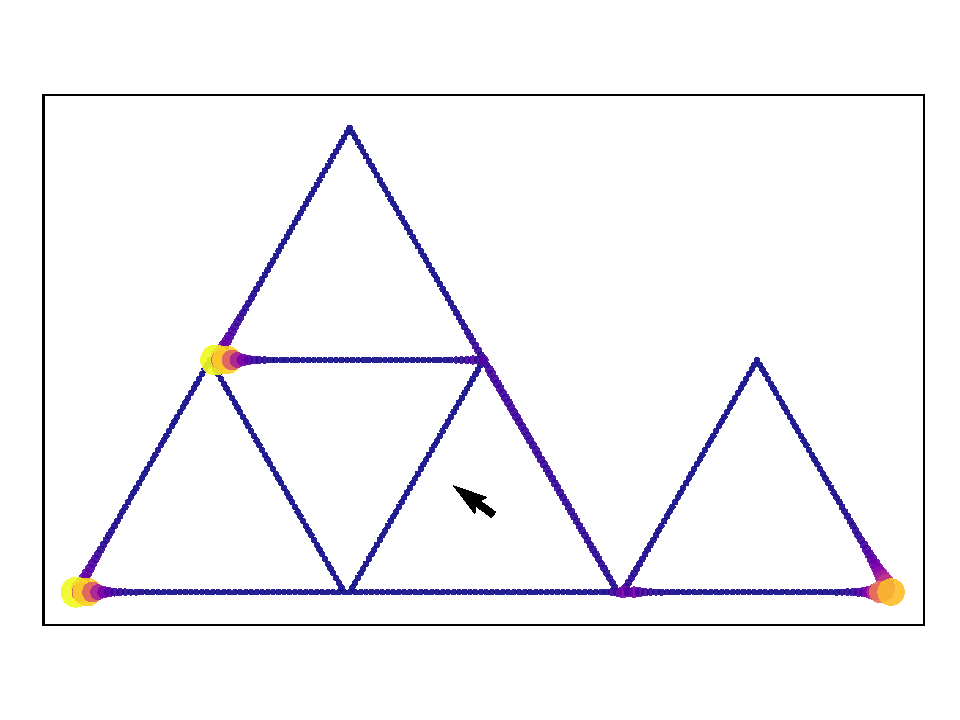
\includegraphics[width=0.30\textwidth]{./figures/supp/GS-T-0_9425.pdf}}
  \subfloat[]{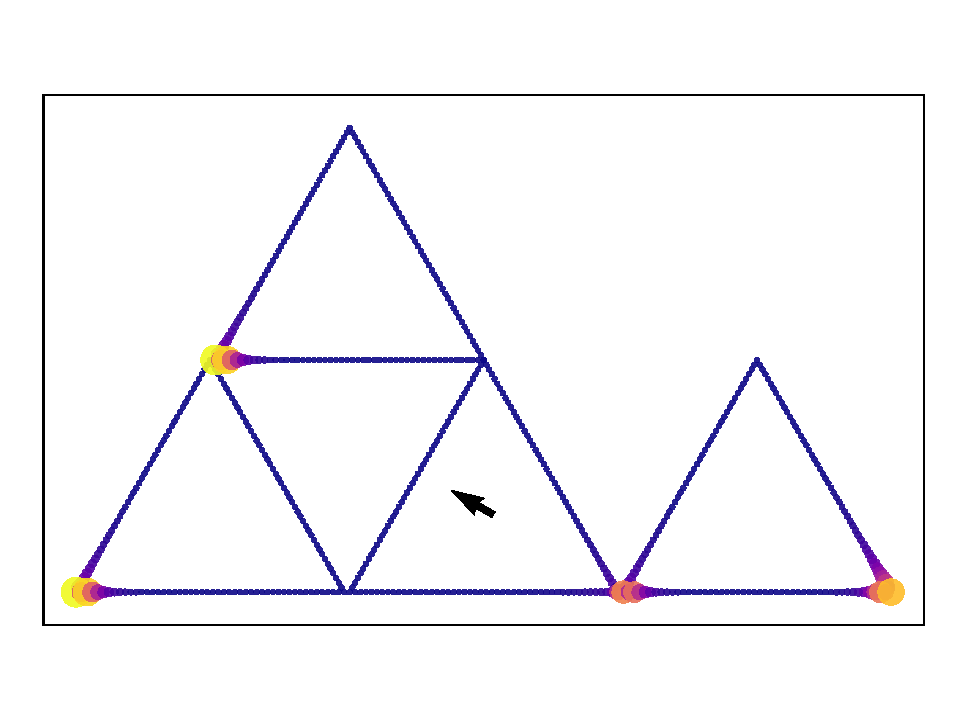
\includegraphics[width=0.30\textwidth]{./figures/supp/GS-T-1_0472.pdf}}
  \caption{(a) Spectral flow for the critical step of swapping $\gamma_2$ and $\gamma_3$ in the example of Fig.~5 in the main text, calculated using four corner-sharing triangles of $W=1$ and $L=50$, with $\mu=1.6$ and $A=2.6$. Vector potential for the middle triangle in the bottom row can rotate according to $\mathbf A = A(-\sin\varphi \hat{x} + \cos\varphi \hat{y})$ from $\varphi = \frac{\pi}{6}$ to $\frac{\pi}{3}$, while the other three have fixed $\varphi = 0$. (b)-(g) BdG eigenfunction $|\Psi|^2$ summed over the four zero modes at equally-spaced points along the rotation path. The black arrow indicates the direction of the vector potential for the bottom middle triangle.}\label{fig: supp braiding}
\end{figure}

In this section we show that one can braid two out of four MZM, a minimal setting for nontrivial manipulation of the degenerate many-body ground states, by using a small network of corner-sharing triangles. We focus on the critical step of swapping $\gamma_2$ and $\gamma_3$ as labeled in Fig.~5 of the main text. This can be done by rotating the vector potential of the triangle in the middle of the bottom row from $\varphi = \frac{\pi}{6}$ to $\frac{\pi}{3}$. More specifically, when $\varphi = \frac{\pi}{6}$, with the chosen values of $\mu$ and $A$, only the right edge of the said triangle is topologically nontrivial. The chain that hosts $\gamma_{3,4}$ thus extends through this nontrivial edge to the top triangle as in Fig.~\ref{fig: supp braiding} (b). On the other hand, when $\varphi$ increases to $\frac{\pi}{3}$, the nontrivial edge of the middle triangle changes from right to left, which leads to $\gamma_2$ hopping from its left corner to the right through the top corner, while $\gamma_3$ is unaffected [Figs.~\ref{fig: supp braiding} (c-g)]. As a result the $\gamma_2,\gamma_3$ swapping is done without closing the bulk gap, as can be seen from the spectral flow in Fig.~\ref{fig: supp braiding} (a).


\section{Discussion}

The hollow interior of the triangles considered in this work is needed for two reasons: (1) $W\ll L$ is required for bulk-edge correspondence based on 1D topology to hold; (2) A finite $W$ is needed to gap out the chiral edge states of a 2D spinless $p$-wave superconductor based on which Eq.~\eqref{eq:Hribbon} is written. The latter is not essential if one does not start with a spinless $p$-wave supercondutor but a more realistic model such as the Rashba+Zeeman+$s$-wave pairing model. On the other hand, the former constraint may also be removed if one uses the Kitaev triangle. Nonetheless, an effective 3-site Kitaev triangle may emerge as the effective theory of triangular structures if a three-orbital low-energy Wannier basis can be isolated, similar to the continuum theory of moir\'{e} structures. We also note in passing that the corner MZM in our triangles appear due to different reasons from that in higher-order topological superconductors \cite{wangEvidenceMajoranaBound2018,pahomiBraidingMajoranaCorner2020}.

\begin{figure}[!hb]
  \begin{tikzpicture}
    \node[inner sep=0pt] (figure) at (0,0)
    {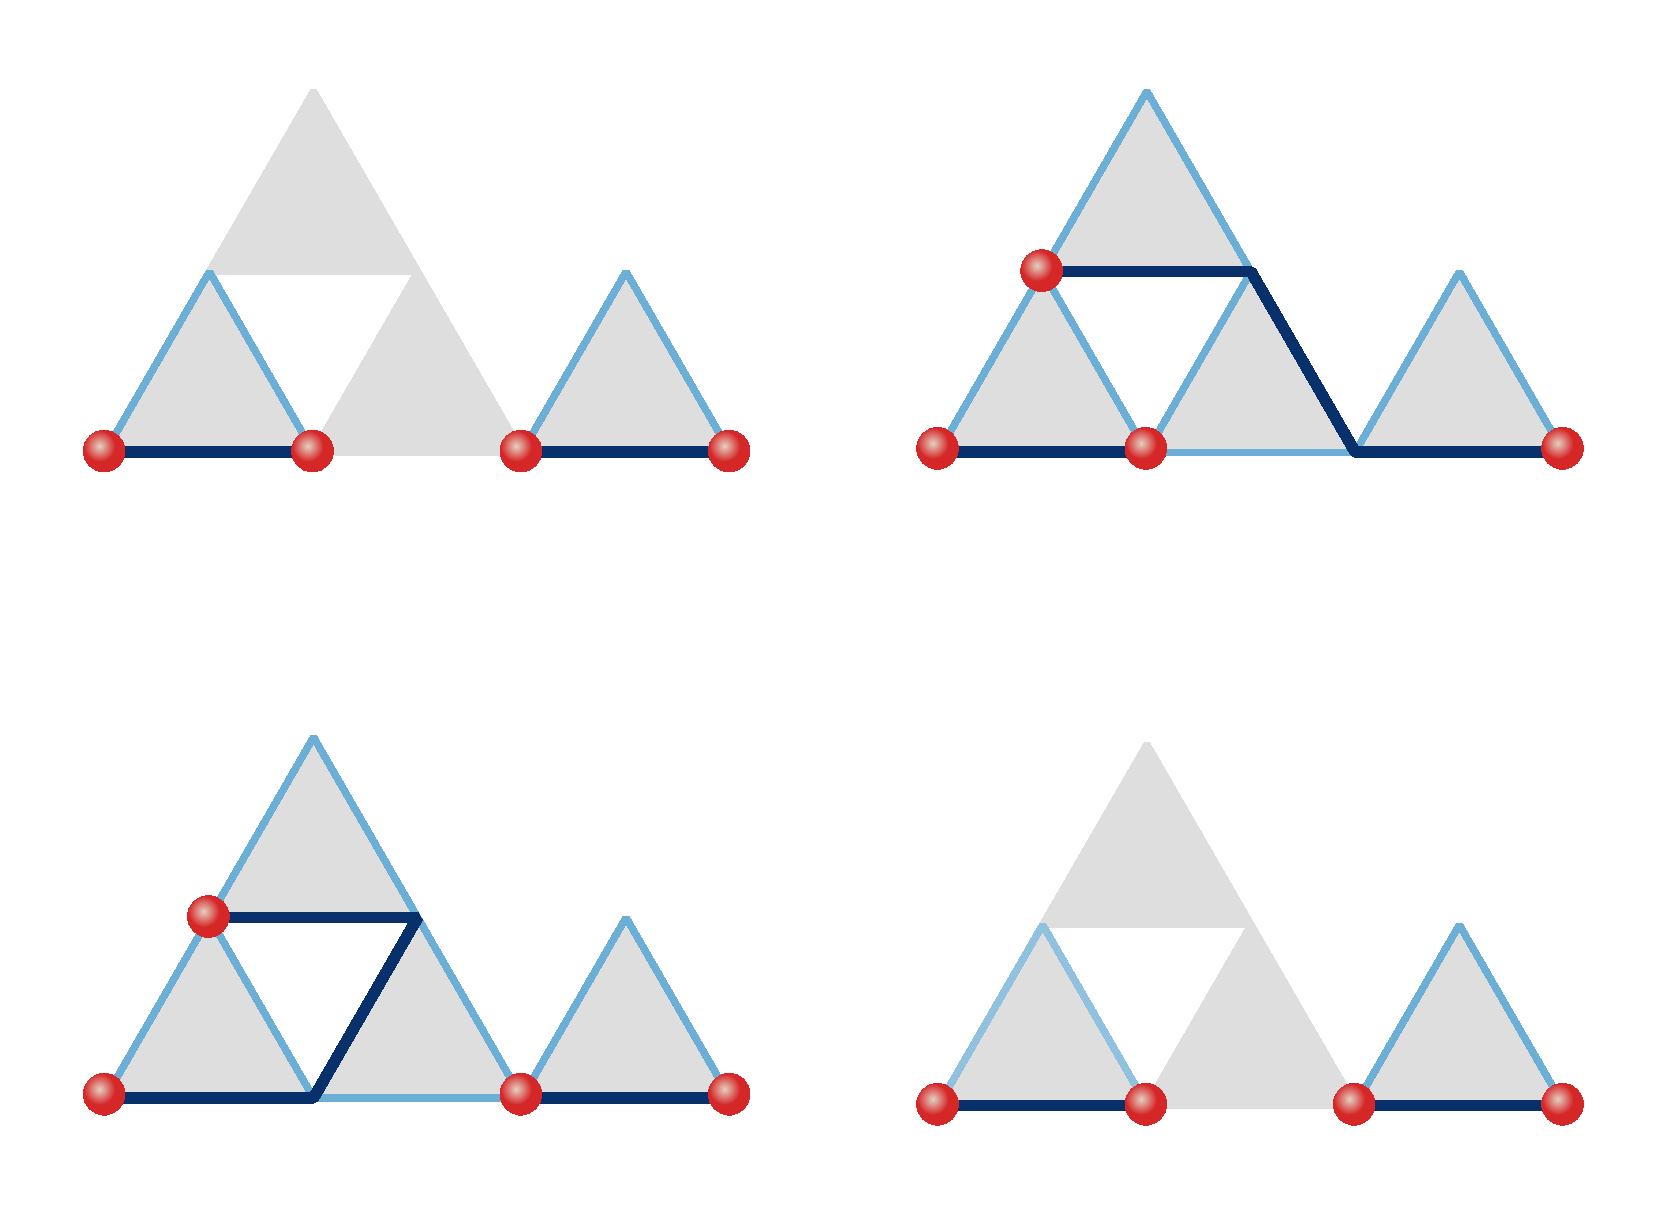
\includegraphics[width=0.90\textwidth]{./figures/4-mf-swap-2-3.pdf}};

    \node[inner sep=0pt] (a) at (-8,5.50) {(a)};
    \node[inner sep=0pt] (b) at (0.2,5.50) {(b)};
    \node[inner sep=0pt] (c) at (-8,-.50) {(c)};
    \node[inner sep=0pt] (d) at (0.2,-.50) {(d)};

    \node[inner sep=0pt] (gamma1) at (-6.6,0.95) {$\gamma_1$};
    \node[inner sep=0pt] (gamma2) at (-4.6,0.95) {$\gamma_2$};
    \node[inner sep=0pt] (gamma3) at (-2.8,0.95) {$\gamma_3$};
    \node[inner sep=0pt] (gamma4) at (-0.9,0.95) {$\gamma_4$};

    \node[inner sep=0pt] (gamma1) at (0.90,0.95) {$\gamma_1$};
    \node[inner sep=0pt] (gamma2) at (2.80,0.95) {$\gamma_2$};
    \node[inner sep=0pt] (gamma3) at (1.4,3.50) {$\gamma_3$};
    \node[inner sep=0pt] (gamma4) at (6.50,0.95) {$\gamma_4$};

    \node[inner sep=0pt] (gamma1) at (-6.6,-4.80) {$\gamma_1$};
    \node[inner sep=0pt] (gamma3) at (-6.0,-2.30) {$\gamma_3$};
    \node[inner sep=0pt] (gamma2) at (-2.8,-4.80) {$\gamma_2$};
    \node[inner sep=0pt] (gamma4) at (-0.9,-4.80) {$\gamma_4$};

    \node[inner sep=0pt] (gamma1) at (0.90,-4.80) {$\gamma_1$};
    \node[inner sep=0pt] (gamma3) at (2.80,-4.80) {$\gamma_3$};
    \node[inner sep=0pt] (gamma2) at (4.60,-4.80) {$\gamma_2$};
    \node[inner sep=0pt] (gamma4) at (6.60,-4.80) {$\gamma_4$};

  \end{tikzpicture}
  \caption{Representative steps for braiding four MZM in four triangles sharing corners. (a) Initialization of four MZM $\gamma_1, \gamma_2, \gamma_3, \gamma_4$. All three edges of the bottom-middle and the top triangles are in the trivial phase by e.g. controlling the chemical potential. The bottom-left and bottom-right triangles have $\varphi = 0$ so that their bottom edges are nontrivial. (b) Moving $\gamma_3$ by ``switching on" the middle triangle by changing the chemical potential under a fixed vector potential at $\varphi=\frac{\pi}{6}$, and then turning on the top triangle with similar means except $\varphi = 0$. (c) Transporting $\gamma_2$ to the right triangle through rotating the vector potential in the middle triangle counterclockwise by $\pi/6$. (d) Moving $\gamma_3$ to the left triangle by ``switching off" the top triangle followed by the middle triangle.}
  \label{fig:4MZMbraiding}
\end{figure}

For possible physical realizations of our triangles, immediate choices are quantum dots forming a Kitaev triangle \cite{dvirRealizationMinimalKitaev2023}, planar Josephson junctions or cuts on quantum anomalous Hall insulator/superconductor heterostructures \cite{xieCreatingLocalizedMajorana2021} that form a hollow triangle, and triangular atomic chains assembled by an STM tip \cite{schneiderPrecursorsMajoranaModes2022} on a close-packed surface. The quantum-dot platform may be advantageous in the convenience of implementing parity readout by turning the third vertex temporarily into a normal quantum dot \cite{mishmashDephasingLeakageDynamics2020,parity_QD_readout_2020, fengProbingRobustMajorana2022}. Looking into the future, it is more intriguing to utilize the spontaneously formed triangular islands in epitaxial growth \cite{pietzschSpinResolvedElectronicStructure2006} with the center region removed either physically by lithography/ablation, or electrically by gating. To create a staggered vector potential or supercurrent profile for the Kitaev triangle, one can use a uniform magnetic field, corresponding to a constant vector potential gradient, plus a uniform supercurrent that controls the position of the zero. It is also possible to use two parallel superconducting wires with counter-propagating supercurrents proximate to the triangle.

A tentative design for braiding more than two MZM, illustrated in Fig.~\ref{fig:4MZMbraiding}, consists of four triangles sharing corners with their neighbors. The critical step of transporting $\gamma_2$ to the left vertex of the rightmost triangle, corresponding to Figs.~\ref{fig:4MZMbraiding} (b,c), can be achieved by rotating the vector potential of the bottom-middle triangle counterclockwisely from $\varphi = \frac{\pi}{6}$ to $\frac{\pi}{3}$, which swaps the topological phases of the two side edges as shown in Fig.~\ref{fig: rotation}. In \cite{supp} we show this operation does not involve gap closing at least for certain parameter regions. Our work provides a versatile platform for manipulating MZM based on currently available candidate MZM systems and for potentially demonstrating the non-Abelian nature of MZM in near-term devices.


\chapter{Floquet Landau Levels}

\begin{enumerate}
  \item \Blue{Introduction (Tahir's intro is fine, maybe in my own words, Floquet engineering)}
  \begin{enumerate}[i]
    \item \Blue{Time dependent, motivation---QAHE gap but not QHE gap}
    \item \Blue{Floquet Theorem--- quasi-energy spectrum}
  \end{enumerate}
  \item \Blue{Results}
  \begin{enumerate}[i]
    \item \Blue{square + \vec{A}(t) (Tahir's perturbative calc)}
    \item \Blue{honeycomb + \vec{A}(t) (Tahir's perturbative calc)}
  \end{enumerate}
  \item \Blue{Discussion and future}
\section{Introduction}

For more than twenty years, Majorana zero modes (MZM) in condensed matter systems have been highly sought after due to their potential for serving as building blocks of topological quantum computation, thanks to their inherent robustness against decoherence and non-Abelian exchange statistics \cite{ivanovNonAbelianStatisticsHalfQuantum2001, kitaevFaulttolerantQuantumComputation2003, nayakNonAbelianAnyonsTopological2008, aliceaNonAbelianStatisticsTopological2011, aasenMilestonesMajoranaBasedQuantum2016}. MZM were originally proposed to be found in half-quantum vortices of two-dimensional (2D) topological \textit{p}-wave superconductors and at the ends of 1D spinless \textit{p}-wave superconductors \cite{readPairedStatesFermions2000, kitaevUnpairedMajoranaFermions2001}. Whether a pristine \textit{p}-wave superconductor \cite{brisonPWaveSuperconductivityDVector2021} has been found is still under debate. However, innovative heterostructures proximate to ordinary $s$-wave superconductors have been proposed to behave as effective topological superconductors in both 1D and 2D. These include, for example, semiconductor nanowires subject to magnetic fields \cite{mourikSignaturesMajoranaFermions2012, rokhinsonFractionalJosephsonEffect2012, dengAnomalousZeroBiasConductance2012}, ferromagnetic atomic spin chains \cite{choyMajoranaFermionsEmerging2011, brauneckerInterplayClassicalMagnetic2013, klinovajaTopologicalSuperconductivityMajorana2013,nadj-pergeProposalRealizingMajorana2013,nadj-pergeObservationMajoranaFermions2014,schneiderPrecursorsMajoranaModes2022}, 3D topological insulators \cite{fuSuperconductingProximityEffect2008, hosurMajoranaModesEnds2011, potterEngineeringMathitipSuperconductor2011, veldhorstMagnetotransportInducedSuperconductivity2013}, quantum anomalous Hall insulators \cite{chenQuasionedimensionalQuantumAnomalous2018, zengQuantumAnomalousHall2018, xieCreatingLocalizedMajorana2021}, quasi-2D spin-orbit-coupled superconductors with a perpendicular Zeeman field \cite{oregHelicalLiquidsMajorana2010, sauGenericNewPlatform2010, lutchynSearchMajoranaFermions2011, potterTopologicalSuperconductivityMajorana2012, liTwodimensionalChiralTopological2016, leiUltrathinFilmsSuperconducting2018}, and planar Josephson junctions \cite{black-schafferMajoranaFermionsSpinorbitcoupled2011, pientkaSignaturesTopologicalPhase2013, hellTwoDimensionalPlatformNetworks2017, fornieriEvidenceTopologicalSuperconductivity2019, renTopologicalSuperconductivityPhasecontrolled2019, scharfTuningTopologicalSuperconductivity2019, zhouPhaseControlMajorana2020}, etc. It has been a challenging task to decisively confirm the existence of MZM in the various experimental systems due to other competing mechanisms that can potentially result in similar features as MZM do in different probes \cite{xuExperimentalDetectionMajorana2015, albrechtExponentialProtectionZero2016, sunMajoranaZeroMode2016, wangEvidenceMajoranaBound2018, jackObservationMajoranaZero2019, fornieriEvidenceTopologicalSuperconductivity2019, renTopologicalSuperconductivityPhasecontrolled2019, mannaSignaturePairMajorana2020}. Other proposals for constructing Kitaev chains through a bottom-up approach, based on, e.g. magnetic tunnel junctions proximate to spin-orbit-coupled superconductors \cite{fatinWirelessMajoranaBound2016}, and quantum dots coupled through superconducting links \cite{sauRealizingRobustPractical2012,leijnseParityQubitsPoor2012,dvirRealizationMinimalKitaev2023} are therefore promising. In particular, the recent experiment \cite{dvirRealizationMinimalKitaev2023} of a designer minimal Kitaev chain based on two quantum dots coupled through tunable crossed Andreev reflections (CAR) offers a compelling route towards MZM platforms based on exactly solvable building blocks.

In parallel with the above efforts of realizing MZM in different materials systems, scalable architectures for quantum logic circuits based on MZM have also been intensely studied over the past decades. A major proposal among these studies is to build networks of T-junctions, which are minimal units for swapping a pair of MZM hosted at different ends of a junction, that allow braiding-based TQC \cite{aasenMilestonesMajoranaBasedQuantum2016}. Alternatively, networks based on coupled wires forming the so-called tetrons and hexons, aiming at measurement-based logic gate operations  \cite{karzigScalableDesignsQuasiparticlepoisoningprotected2017}, have also been extensively investigated. To counter the technical challenges of engineering networks with physical wires or atomic chains, various ideas based on effective Kitaev chains, such as quasi-1D systems in thin films \cite{potterMultichannelGeneralizationKitaev2010}, cross Josephson junctions \cite{zhouPhaseControlMajorana2020}, scissor cuts on a quantum anomalous Hall insulator \cite{xieCreatingLocalizedMajorana2021}, and rings of magnetic atoms \cite{liManipulatingMajoranaZero2016}, etc. have been proposed. However, due to the same difficulty of obtaining or identifying genuine MZM in quasi-1D systems mentioned above, it remains unclear how practical these strategies are in the near future.

In this Letter, we propose an alternative structural unit for manipulating MZM, triangular superconducting islands, motivated by the above challenges associated with wire geometries and by the fact that triangular islands routinely appear spontaneously in epitaxial growth \cite{pietzschSpinResolvedElectronicStructure2006} on close-packed atomic surfaces. We first show that a minimal ``Kitaev triangle'' consisting of three sites hosts MZM at different pairs of vertices controlled by Peierls phases on the three edges [Fig.~\ref{fig:triangles} (a)], which can be readily realized using quantum dots. To generalize the minimal model to triangular structures involving more degrees of freedom, we study the topological phase transitions of quasi-1D ribbons driven by Peierls phases, which can be created by magnetic fields or supercurrents \cite{romitoManipulatingMajoranaFermions2012, takasanSupercurrentinducedTopologicalPhase2022}, and use the resulting phase diagram as a guide to construct finite-size triangles with a hollow interior that host MZM  [Fig.~\ref{fig:triangles} (b)]. In the end we discuss possible experimental systems that can realize our proposals and scaled-up networks of triangles for implementing braiding operations of MZM.



\section{Floquet Landau level-like bands in Dirac systems}
In this section we demonstrate a Dirac system in the presence of a standing, non-uniform, circularly polarized light becomes an effective Dirac Hamiltonian with a magnetic field that is composed of the electric field component of light.
Dirac electrons can be represented with a generic model 2D Hamiltonian honeycomb monolayer in the presence of a gauge potential as

\begin{figure}
  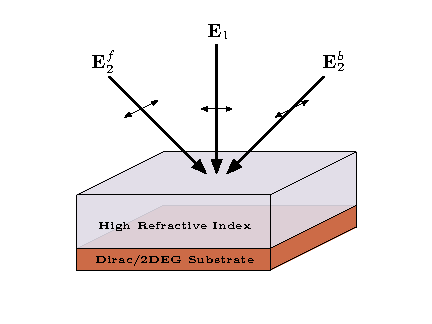
\includegraphics[width=0.5\textwidth]{./figures/fll-setup.pdf}
  \caption{Schematic of two oblique (forward and backward) and one normally incident light on graphene or a 2DEG substrate with high refractive index material on top. Oblique lasers have polarization in $y$-axis and travel in $xz$-plane and normally incident laser has polarization in the $x$-axis and travel in $yz$-plane. With beam width large enough to cover the device fully.}
  \label{fig:fll-setup}
\end{figure}

\begin{equation}\label{eq:HDirac}
  \ham(t) = v_{F} \bm{\sigma} \cdot \left(\vec{p} + e\vec{A}(t)\right),
\end{equation}
where $\vec{A}$ is the gauge potential, $\vec{p}$ is the momentum operator, $v_F$ is the Fermi velocity of Dirac fermions, $e$ is electron charge, and $\vec{\sigma}$ the Pauli matrices vector in 2D.
The light is made of three linearly polarized lasers, as shown in Fig. \ref{fig:fll-setup}.
Where the first is normally incident in the $z$-axis with polarization in the $x$-axis.
The second and third are of oblique incidence in the $xz$-plane, to acquire non-uniformity in the $x$-axis, with polarization in the $y$-axis, and mirrored about the $yz$-plane.
This is to introduce $x$-dependence with the $p_y$ term of the Dirac Hamiltonian.
The relevant electric field components at the Dirac system interface are

\begin{align} \label{eq:EDfield}
\vec{E}_{1} &= E\cos \omega t\ \hat{x}, \nonumber \\
\vec{E}_{2} &= \vec{E}_2^f + \vec{E}_2^b = E\sin(Kx)\sin 2\omega t\ \hat{y},
\end{align}
%Where $\omega$ is angular frequency of light with time $t$ and $K=2\pi /d$ with $d$ being the spatial period of the electric field with amplitude $E$.
Where $\omega$ is angular frequency of the laser with time $t$ and $K = \omega \sin{(\theta_i)} / v_p$, with $\theta_i$ as incident angle of the oblique lasers and $v_p$ is phase velocity of the lasers.
%Notice, the second electric field has twice frequency of the first, this is a requirement to make the Dirac Hamiltonian into a Landau level-like Hamiltonian, the derivation in REFERENCE APPENDIX can inform the reader of this choice.
Notice, the second electric field has twice frequency of the first, this allows for the second gauge potentials $\sigma_y$ to have non-zero commutation with the first gauge potentials $\sigma_x$, and due to the high-frequency expansion used later, allows for the second gauge potential to return to a $\sigma_y$, as seen in \ref{fll-dirac-derivation}.
This form of the electric field relates to the following gauge potential, via $\vec{E} = -\partial_t \vec{A}$ as

\begin{equation}\label{eq:ADirac}
  \vec{A}(t)= \dfrac{E}{\omega} \left\langle -\sin \omega t, \tfrac{1}{2}\sin(Kx) \cos 2\omega t \right\rangle,
\end{equation}%
Substituting Eq.~\eqref{eq:ADirac} into Eq.~\eqref{eq:HDirac}, we arrive at%

\begin{equation}\label{eq:HDtime}
  \ham(t)= v_{F}\bm{\sigma}\cdot\vec{p} - \sigma _{x} \dfrac{v_F eE}{\omega} \sin {\omega t} - \sigma _{y} \dfrac{v_F eE}{2\omega}\sin{(Kx)} \cos2\omega t.
\end{equation}%
Due to the laser's time-translation symmetry through $A(t+T)=A(t)$ with $T=2\pi /\omega $, one can apply the Floquet theory \cite{AEE, MBL, supp} and obtain an effective Hamiltonian from Eq.~\eqref{eq:HDtime}.
This introduces the quasienergy matrix $Q_{m,m+n} = H_n + m\hbar\omega\delta_{n0}$ after performing the Fourier time-transform of the Hamiltonian, given as

\begin{equation} \label{eq:fourier-time-transform}
  H_n = \dfrac{1}{T} \int_{0}^{T} \ham(t) e^{-in\omega t} dt,
\end{equation}
then we are left with modes $m=0,\pm1,\pm2$.
To use the high-frequency approximation we require $\hbar\omega \gg H_{\pm1,\pm2}$, the off-diagonal terms.
After applying the high-frequency approximation to first and second order expansion in $\hbar\omega$, it leads to the zeroth-mode effective Hamiltonian in Eq.~\eqref{eq:HDtime} as

\begin{equation} \label{eq:HDeff}
  H_{\text{eff}}= v_{F}\bm{\sigma}\cdot\vec{p}-\sigma_y\frac{v_F^3 e^2 E^2 p_y}{\hbar^{2}\omega^{4}}
  +\sigma_y\frac{v_F^3 e^3 E^{3}\sin{(Kx)}}{4\hbar^{2}\omega^{5}}
  -\sigma_x\frac{v_F^3 e^2 E^2 \left\{p_x, \sin^2{(Kx)} \right\} }{8\hbar^{2}\omega^{4}}.
\end{equation}
The derivation can be found in the Appendix \ref{fll-dirac-derivation}.
This effective Hamiltonian can be simplified in the long wavelength limit, $Kx \ll 1$ to

\begin{align} \label{eq:HeffDirac}
  %\ham_{\text{eff}} &= v_F \sigma_x p_x + v_F \sigma_y \left[ \left( 1- \dfrac{v_F^2e^2E^2}{\hbar^2\omega^4} \right) p_y + \dfrac{K v_F^2 e^3 E^3}{4 \hbar^2 \omega^5} x \right] \nonumber \\
  \ham_{\text{eff}}^D &= v_{F}\sigma_{x}p_{x}+v_F\sigma_{y} \left( C p_{y} + eB^Dx \right),
\end{align}%
where $C = 1-\left(\tfrac{v_{F}eE}{\hbar\omega^2}\right)^2$ and $B^D=\frac{Kv_F^2 e^2E^3}{4\hbar^{2}\omega^{5}}$.
%In accordance with Eqs.~\eqref{eq:HDeff} and ~\eqref{eq:HeffDirac}, there is least anisotropy in the Dirac spectrum in addition to zero gap.
Diagonalizing the Hamiltonian in Eq.~\eqref{eq:HeffDirac}, we obtained the eigenvalues for Dirac system as%

\begin{equation} \label{eq:DiracEner}
  \epsilon_{n}^D = \pm v_F^2 \sqrt{\dfrac{nK e^3 E^3}{2 \hbar \omega^5}}
\end{equation}
which is similar to graphene LLs spectrum in the limit of equal velocities.
The effective magnetic field in the Dirac Hamiltonian achieves a highly degenerate energy spectrum similar to LLs.
Unlike conventional LLs, the electron motion is not a cyclotron orbit but a potentially more complicated orbit, due to CPL inducing a Coulumb force in the material's 2D plane.
In Eq. ~\eqref{eq:HDeff}, the first order term in $\hbar \omega$ leads to gap at the Dirac point in normally incident, circularly polarized light experiments \cite{YHW, JWM} and is zero here due to the non-uniformity nature of oblique incident lasers.

There are several ways to enhance the effective magnetic field and directly LL-like energies for a Dirac system.
Electric field strength can be increased within reason as we are limited by the photon energy to ensure the high-frequency expansion holds, $E \ll 2\hbar\omega^2/e v_F$.
One can reasonably use electric field strengths up to 20\% of the limit due to photon energy.
The laser wavenumber $K= \omega \sin{(\theta_i)} / v_p$ has a linear relationship to photon energy, too.
Overall, considering the high-frequency limit on the electric field, the effective field $B^D \propto \omega^2 \sin{(\theta_i)} / (v_F v_p)$.
Without too much consequence the incident angle can be increased up to $\pi/2$ and decreasing the phase velocity of light would enhance the effective magnetic field.
Increasing photon energy is one way to enhance the effective magnetic field.
As considered in previous literature, when photon energy and electric field are increased more energy is pumped into the system, shorter pulses are required to prevent damaging the system \cite{YHW, JWM}.

%\Blue{This next paragraph should be in the discussion since it uses similar language and results as 2DEG?}
%It is important to note, that this system experiences QHE for values of $C\neq0$ and can flip chirality when $C$ changes sign, more details in REFERENCE APPENDIX.
%We can have gapped Dirac spectrum and QAHE by using uniform circularly polarized laser light as observed in experiments \cite{YHW, JWM} or by using any substrate like hBN.
%Now, we have shown one can achieve a highly degenerate Landau level-like spectrum and QHE with an effective magnetic field strength which is directly proportional to third order of the electric field and inversely proportional to the product of spatial period and fifth order of the frequency of the polarized light $\propto (E^3/(d\omega^5))$.
%This factor of the laser lights can be tuned and thus effective magnetic field can be enhanced in such nonequilibrium systems.
%In the case of uniform circularly polarized light, one can imagine the Coulomb force makes the charged particles move in a cyclotron orbit.
%In constrast, for non-uniform circularly polarized light, charged particles are not necessarily in cyclotron orbits but in some form of closed orbit preventing the charged particles from moving on average in a given direction, hence we define them as Landau level-lik.

\section{Floquet LLs in 2DEG}
We consider the case of Schr\"{o}dinger electrons under the application of two linearly polarized laser lights. The unperturbed Hamiltonian for 2DEG is%
\begin{equation}\label{eq:H2DEG}
H=\frac{\pi_{x}^{2}}{2m^{\ast}}+\frac{\pi_{y}^{2}}{2m^{\ast}},
\end{equation}
where $m^{\ast}$ is the effective mass of electron. By changing the Hamiltonian into a time-dependent form by applying two linearly polarized lights
such that $\bm{\pi}\rightarrow \vec{p}-q\vec{A}(t)$. \ Therefore, Eq.~\eqref{eq:H2DEG} is written as%
\begin{equation}\label{eq:H2time}
H(t)=\frac{1}{2m^{\ast}}[p_{x}-qA_{x}(t)]^{2}+\frac{1}{2m^{\ast}}[p_{y} -qA_{y}(t)]^{2},
\end{equation}
where the electric field components for two spatially inhomogeneous linearly polarized laser lights are
\begin{align} \label{eq:E2field}
  \vec{E}_{1} &= E\sin{(Kx)} \cos{(\omega t)}\hat{x}, \nonumber \\
  \vec{E}_{2} &= -E\sin{(Kx)} \sin{(\omega t)}\hat{y}.
\end{align}%
The field given in Eq.~\eqref{eq:E2field} lead to the following vector potential $\vec{A}(t)$
\begin{equation}\label{eq:Avec2deg}
  \vec{A}(t)= -\dfrac{E}{\omega} \sin{(Kx)} \left\langle \sin (\omega t), \cos{(\omega t)},0 \right\rangle.
\end{equation}%
Substituting into the Schrodinger Hamiltonian we arrive at

\begin{align}\label{eq:Htime2deg}
  \ham(t) = \dfrac{1}{2m} [ &p_x^2 + p_y^2 + V^2 \sin^2{(Kx)} + V^2 \sin{(\omega t)} (p_x \sin(Kx) + \sin(Kx) p_x) + 2Vp_y \sin(Kx) \cos(\omega t) ]
\end{align}
where $V=qE/\omega$.
Because of the time-translation symmetry through $A(t+T) = A(t)$ with $T = 2\pi/\omega$, one can apply the Floquet theory \cite{AEE, MBL, supp} and obtain an effective Hamiltonian from Eq.~\eqref{eq:Htime2deg}. After performing the Fourier transform of the time-periodicity, first order expansion in $\hbar \omega$ terms and in the long wavelength limit leads to the final effective Hamiltonian as

\begin{align}\label{eq:Heff2deg}
  \ham_{\rm eff} &= \dfrac{1}{2m} \left[ p_x^2 + p_y^2 + V^2K^2x^2 + \dfrac{\hbar V^2}{4m\omega} (K^2 - 2K^4x^2) - \dfrac{2V^2K^2}{m\omega} p_y x \right] \nonumber \\
  \ham &= \dfrac{1}{2m} \left[ p_x^2 + p_y^2 - \dfrac{2V^2K^2}{m\omega} p_y x + \left(1-\dfrac{\hbar K^2}{2m\omega}\right)V^2K^2x^2 + \dfrac{\hbar V^2 K^2}{4m\omega} \right]
\end{align}
Notice here we have quantum harmonic oscillator (QHO) in x-axis and also coupling between $p_y$ and $x$.
The coupling can allow for flux pumping.
While we may have Landau levels, from the QHO, it still needs to be shown if our system has topological edge states.

\subsection{2DEG Numerical Approach}

We now consider a 2D square lattice tight-binding model.
The incident laser light doesn't allow for translation symmetry along the x-axisin which we will only consider a finite radius along the x-axis and treat the y-axis as infinite.
Our unit cell will still only contain one atom per cell, this will not be the case for Dirac.
Lattice vectors are described as follows $\vec{a}_1 = a\hat{x}$, and $\vec{a}_2 = a \hat{y}$.
We will use a Peierls phase to introduce the vector potential field to the tight-binding Hamiltonian.
In general, the Hamiltonian has the following form:
\begin{equation}
  \ham(t) = -\sum_{jl} h_{j,j+1}(t) \cc_{j,l} c_{j+1,l} + h_{l,l+1} \cc_{j,l} c_{j,l+1} + h.c.
\end{equation}
where $h$, hopping amplitude, takes the following phase contributions

\begin{align}
  h_{j,j+1}(t) &= \exp \left[ i \dfrac{qE}{\hbar \omega}(x_{j+1}-x_j) \sin(K\bar{x}_{j,j+1}) \sin{\omega t} \right] \nonumber \\
  h_{j,j+1}(t) &= \exp \left[ i Z_1 \sin{\omega t} \right] \\
  h_{j+1,j}(t) &= \exp \left[ -i Z_1 \sin{\omega t} \right] \\
h_{l,l+1}(t) &= \exp \left[ i \dfrac{qE}{\hbar \omega} (y_{l+1}-y_l) \sin(Kx_j) \cos\omega t \right] \nonumber \\
  h_{l,l+1}(t) &= \exp \left[ i Z_2 \cos\omega t \right] \\
  h_{l+1,l}(t) &= \exp \left[ -i Z_2 \cos\omega t \right]
\end{align}
where $Z = qEa/\hbar \omega$, $Z_1 = Z\sin(K\bar{x}_{j,j+1})$, $Z_2 = Z\sin(Kx_j)$, and $\bar{x}_{j,j+1} = (x_{j+1}+x_j)/2$.
One can fourier transform along the y-axis to momentum space to simplify the system to

\begin{align}
  \ham(t) &= -\sum  h e^{iZ_1\sin{\omega t}} \cc_{jk} c_{j+1,k} + h e^{ i Z_2 \cos(\omega t) - ika} \cc_{jk} c_{jk} + h.c. \nonumber \\
  &= -\sum_{jk} h_{j,j+1}(t) \cc_{jk} c_{j+1,k} + h_{jk}(t) \cc_{jk} c_{jk} + h.c.
\end{align}

We next impose Floquet theory and take fourier time-domain transforms of the Hamiltonian.
Both of the terms take the following form

\begin{align}
  h_{j,j+1,n} &= \dfrac{1}{T} \int_0^T h_{j,j+1}(t) e^{-in\omega t} dt \nonumber \\
  &= \dfrac{h}{T} \int_0^T e^{iZ_1 \sin{\omega t} -in\omega t} dt \nonumber \\
  &= \dfrac{h}{2\pi} \int_0^{2\pi} e^{iZ_1 \sin\tau - in\tau} d\tau \nonumber \\
  &= h J_n(Z_1) \\
  h_{j+1,j,n} &= h (-1)^n J_n(Z_1)
\end{align}

\begin{align}
  h_{jk,n} &= \dfrac{1}{T} \int_0^T h_{jk}(t) e^{-in\omega t} dt \nonumber \\
  &= \dfrac{h}{T} e^{-ika} \int_0^T e^{- iZ_2 \cos{(\omega t)} - in\omega t} dt \nonumber \\
  &= \dfrac{h}{2\pi} e^{-ika} \int_0^{2\pi} e^{-i Z_2\cos\tau - in\tau} d\tau \nonumber \\
  &= \dfrac{h}{2\pi} e^{-in\pi/2-ika} \int_0^{2\pi} e^{-iZ_2 \cos\tau - in\tau + in\pi/2} d\tau \nonumber \\
  &= he^{- in\pi/2 -ika} J_{n}(Z_2) \\
  h_{jk,n}^* &= he^{+ in\pi/2 +ika} J_{n}(Z_2)
\end{align}
The Hamiltonian after fourier transform is

\begin{equation}
  H_n = -h \sum_{jk} J_n(Z_1) \left(\cc_{jk} c_{j+1,k} + (-1)^n \cc_{j+1,k} c_{jk}\right) + 2\cos\left(ka+\tfrac{n\pi}{2}\right) J_n(Z_2) \cc_{jk} c_{jk}
\end{equation}

We now build the quasienergy matrix $\bar{Q}$ that has matrix elements

\begin{equation}
  \bar{Q}_{m,m+n} = H_n - m\hbar\omega \delta_{n0}
\end{equation}
The quasienergy matrix by definition is infinite in Floquet theory and thus not possible to solve at least numerically.
However, since we are interested in the behavior at zeroth mode and depending on the stregnth of laser light energy, $\hbar\omega$, we choose a cutoff mode $|m|\leq m_c$, where $m_c$ is a positive integer such that higher modes do not contribute to the zeroth modes behavior.
Notice we have two cutoffs, one for x-axis radius and for light modes.
This translates to a matrix with dimensions ${(N_r N_m)}^2$, $N_r = (2*r_c+1)$, and $N_m=(2*m_c+1)$.


\section{Conclusion}

We now examine the topology of both systems.
Eqs. \eqref{eq:HeffDirac} and \eqref{eq:Heff2deg} are in LL Hamiltonian form, and typically exhibit QHE.
The two systems only have translational symmetry in the $y$-axis, so a Chern number based on periodicity in $k_x$ and $k_y$ is not applicable, though one can relate the center of mass of an electron to the Chern number as shown in Appendix \ref{chern-number}, which is related to the Laughlin pump.
Considering the Laughlin pump argument, both systems have quantized Hall conductivity, since both have the same eigenstates as their respective LL Hamiltonian.
A key difference to note about both systems is the $C$ term in Eq. \eqref{eq:HeffDirac}.
This term will stay positive for the values of $E$ used in the high-frequency limit for the Dirac case.

Using existing experiments \cite{YHW, JWM} we can provide an estimate for the strength of the effective magnetic field to observe LL-like spectrum and QHE.
Analytical structure of Eq.~(\ref{eq:DiracEner}) and Eq.~(\ref{eq:2DEGenergy}) is primarily responsible for the LL-like spectrum in both the Dirac and 2DEG systems, respectively.
Although such results are valid for other 2D materials or Schr\"{o}dinger systems, however, for simplicity, we will consider parameters realized for graphene or topological insulators \cite{YHW, JWM}.
We will consider a similar range of mid-IR photon energies (or $\lambda = [3\mu $m$ , 10\mu $m$]$) as seen in graphene or topological insulators \cite{YHW, JWM} to match with recently proposed high refractive index metamaterial composites \cite{shimFundamentalLimitsRefractive2021}.
In these experiments \cite{YHW, JWM}, the strength of the electric field used is $1 \times 10^7$ V/m to $1 \times 10^8$ V/m, for the parameters used to estimate effective magnetic fields for both systems the largest electric field is around $1.4 \times 10^8$ V/m.
As should be considered, the larger both photon energy and electric field become ultrafast pulses should be used to prevent thermal damage to materials, on the order of $500$ fs.
To note, for the following results we assume a high oblique angle to let $\sin{(\theta_i)} \approx 1$.

To enhance the effective magnetic field, aside from using higher photon energy, reducing the photon phase velocity can see a considerable increase in both systems.
The refractive index materials can be set above graphene, or any Dirac material, such that the laser light can propagate through to reduce its phase velocity.
Germanium refractive index increases monotonically with increasing photon energy, we use a linear interpolation of the refractive index due the small change for the range of photon energies used.
Al-composite metamaterials refractive index is monotonically decreasing with increasing photon energy and we use a linear interpolation here as the data is roughly linear.

\begin{figure}
  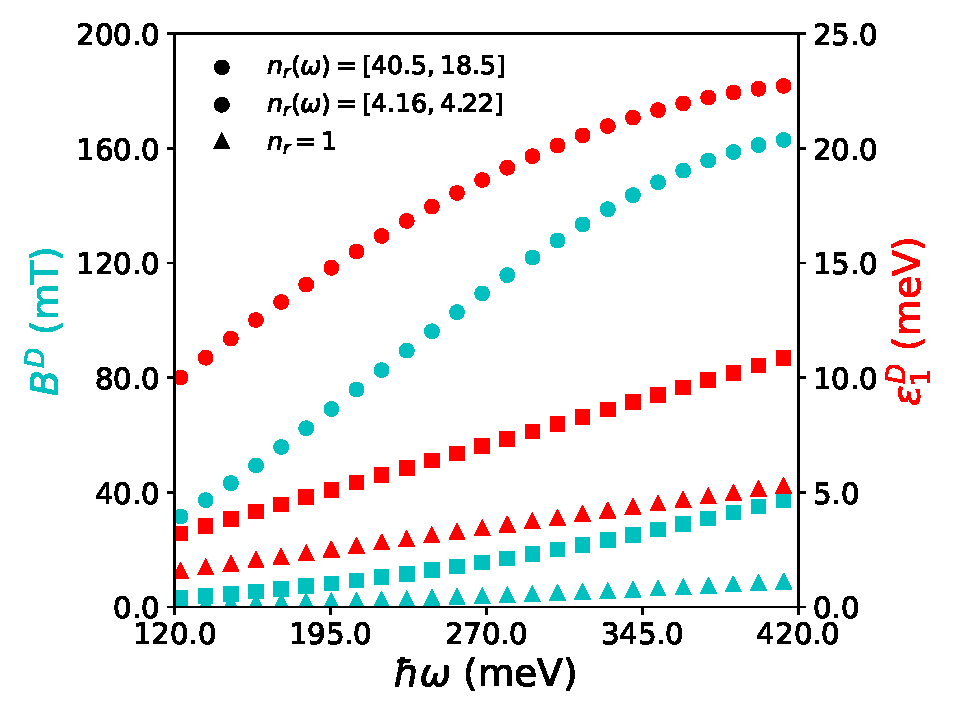
\includegraphics[width=0.45\textwidth]{./figures/dirac-eff-bfield-energy.pdf}
  \caption{Effective magnetic field (cyan) and first quasienergy (red) as a function of photon energy for various refractive materials: vacuum (triangles), germanium (squares), and  Al-composite metamaterial (circles).}
  \label{fig:dirac-bfield-energy}
\end{figure}

In case of a Dirac system Fig. \ref{fig:dirac-bfield-energy} shows graphene with various refractive index materials to enhance the effective magnetic field and first order quasienergy of the LL-like spectrum.
For mid-IR ranges of laser light, the effective magnetic field (cyan) can get up to $8.8$ mT for vacuum, $37.2$ mT for germanium, and $163$ mT for Al-composite metamaterial for $\hbar\omega=413$ meV and results in first order quasienergies (red) of $5.3$ meV, $11$ meV, and $23$ meV, respectively.
As can be seen in \ref{fig:dirac-bfield-energy} as photon energy increases the Al-composite refractive index decreases quite a bit and if we used higher energy we would see the effective magnetic field and quasienergies start to decrease, as will be seen with 2DEG.
While the material has higher index of refraction overall, it would be better to find a material that increases refractive index with photon energy, like germanium can, for it can drastically increase for slightly higher photon energies before effective magnetic field dips \cite{amotchkinaCharacterizationEbeamEvaporated2020}.

\begin{figure}
  \subfloat[]{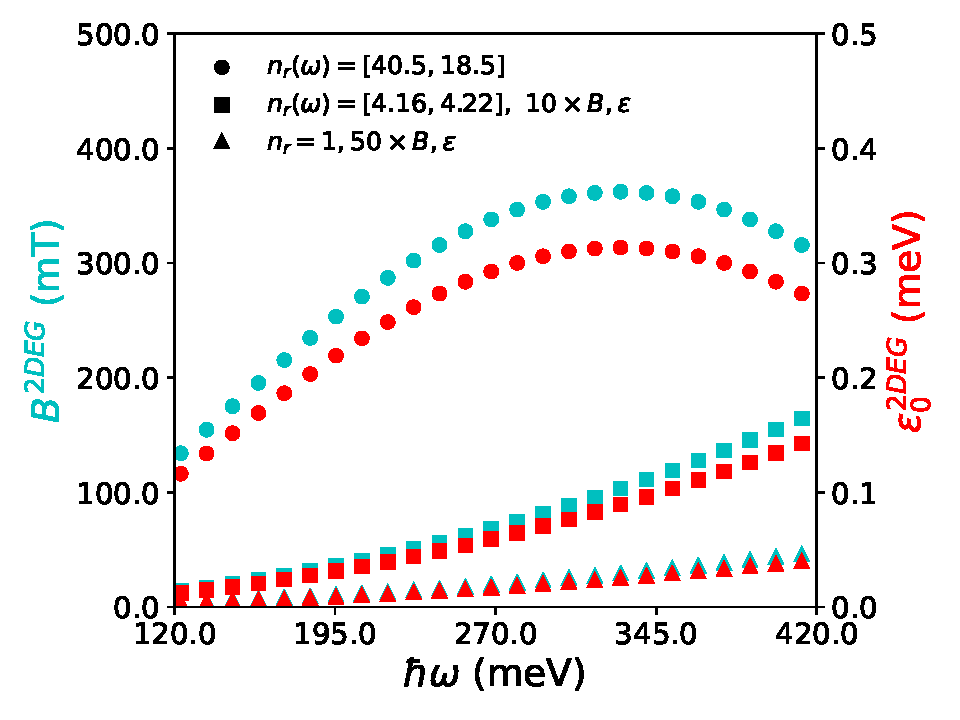
\includegraphics[width=0.45\textwidth]{./figures/2deg-eff-bfield-energy-GaAs.pdf}}
  \subfloat[]{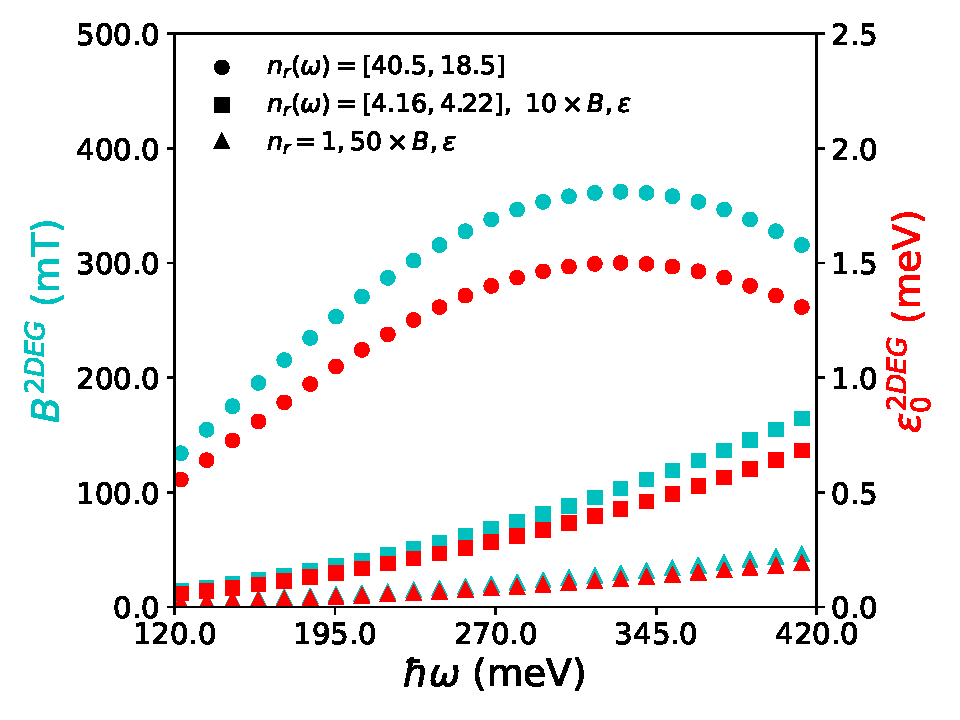
\includegraphics[width=0.45\textwidth]{./figures/2deg-eff-bfield-energy-InSb.pdf}}
  \caption{Effective magnetic field (cyan) and first quasienergy (red) as a function of photon energy for 2DEGs for various refractive materials: vacuum (triangles) scaled by a factor of 50, germanium (squares) scaled by a factor of 10, and Al-composite metamaterials. The 2DEG materials used are (a) GaAs and (b) InSb.}
  \label{fig:2deg-bfield-energy}
\end{figure}

For 2DEG systems Fig. \ref{fig:2deg-bfield-energy} shows GaAs and InSb materials with the same refractive materials used for graphene to enhance effective magnetic field and zeroth order quasienergy of the LL-like spectrum.
The vacuum and germanium interfaces are scaled up by a factor of $10$ and $50$, respectively, to visually enhance and compare it to the Al-composite interface.
GaAs is used as it is one of the most common 2DEG with relatively small effective electron mass, followed by InSb since it has the smallest effective electron mass found in 2DEG materials.
For the GaAs system, effective magnetic field (cyan) can get up to $0.92$ mT for vacuum, $16.5$ mT for germanium, and $362$ mT for Al-composite metamaterial and achieves zeroth order quasienergies (red) of $0.8\ \mu$eV, $14.3\ \mu$eV, and $314\ \mu$eV, respectively.
In the InSb system, effective magnetic field is the same as GaAs, since it has no dependence on effective mass, and achieves zeroth order quasienergies (red) of $3.8\ \mu$eV for vacuum, $68.2\ \mu$eV for germanium, and $1.5$ meV for Al-composite.
As alluded to earlier, due to Al-composites large decrease in refractive index for increasing photon energy, it peaks earlier around $\hbar\omega=328$ mT, for 2DEG.
Overall, we see large changes in 2DEG for both effective magnetic field, due to being proportional to refractive index squared and quasienergies, being inversely proportional to effective electron mass.

There are a few items we did not consider for our calculations.
First, we do not consider any effects due to a refractive index material in contact with a Dirac or 2DEG system.
Secondly, while the high-frequency expansion limits the electric field applied to the materials one could still go beyond the limit of $\hbar \omega \ll H_{pm1}, H_{\pm2}$ to enhance the effective magnetic field by a few orders of magnitude with some error.
For example, if instead we use $\hbar\omega = H_{\pm1}, H_{\pm2}$, this would be multiplying the electric field by a factor of $5$ from our calculations presented, Dirac effective magnetic field would increase by a factor of $125$ while 2DEG effective magnetic field would increase by a factor of $25$.
For Dirac systems with higher electric field strengths, if $C=0$, there would be no QHE as there is no coupling between $x$ and $p_y$, and if $C<0$, the direction of chirality flips.

In conclusion, we have shown Floquet LLs and the QHE using three linearly polarized lights for Dirac and conventional 2DEG systems.
While using these laser lights, we  need at least two polarized lights to be spatially inhomogeneous and mirrored.
We have presented results using frequency space expansion method and degenerate Floquet perturbation theory.
While, a tight-binding model capable of using ``low-frequency'' with a Peierls substitution can be found in appendix \ref{app:tbm-dirac} and \ref{app:tbm-2deg}, the results are difficult to interpret and currently not informative.
The results agree well to show Floquet LL-like energies in experimentally accessible parameters range.
Also, it is vital to note we are flexible to use different values of the electric field strength, photon energy, or phase velocity to realize QHE and control the strength of the effective magnetic field.
Therefore, we think Floquet LL-like and QHE can be observed in experiments for moderate strength of the spatially inhomogeneous laser lights. Moreover, we expect to open up new avenues for nanoelectronics in nonequilibrium systems.



\end{enumerate}

\chapter{Conclusion and Discussion}

\Blue{What makes gauge potential unique in creating/tuning/manipulating new topoglical systems}
\Blue{Applications}

\begin{appendices}
\chapter{Suitable Name}
\begin{enumerate}
  \item \Blue{Majorana Number derivation}
  \item \Blue{Other derivations not included in introduction}
\end{enumerate}
\section{Kitaev Triangle and Peierls substitution}

We start with a spinless or spin-polarized \textit{p}-wave superconductor

\begin{equation}
  \ham = \sum_{\langle j, l \rangle} (-t\cc_{j} c_l + \de e^{i\theta_{jl}} c_{j} c_l + h.c.) - \sum_j \mu \cc_j c_j,
\end{equation}
where $t$ is the hopping amplitude, $\de$  is the amplitude of (2D) \textit{p}-wave pairing, $\mu$ is the chemical potential, $\theta_{jl}$ is the polar angle of $\vec{r}_{jl} = \vec{r}_l - \vec{r}_j$, consistent with $\{\cc_l, \cc_j\} = 0$.

We will now include a gauge potential via a Peierls substitution as
\begin{align}\label{eq:HBdG}
  \cc_j &\rightarrow \cc_j \exp(-\dfrac{i e}{\hbar} \int_0^{\vec{r}_j} \vec{A} \cdot d\vec{l}), \nonumber \\
  \cc_j c_l &\rightarrow \cc_j c_l \exp(\dfrac{i e}{\hbar} \int_{\vec{r}_j}^{\vec{r}_l} \vec{A} \cdot d\vec{l}) \nonumber \\
  &\rightarrow \cc_l c_j e^{i \phi_{j,l}}. \nonumber \\
  \phi_{jl} &= \dfrac{e}{\hbar} \int_{\vec{r}_j}^{\vec{r}_l} \vec{A} \cdot d\vec{l} = -\phi_{lj}
\end{align}

The modified Hamiltonian is then
\begin{equation}
  \ham = \sum_{\langle j, l \rangle} (-t e^{i\phi_{jl}} \cc_{j} c_l + \de e^{i\theta_{jl}} c_{j} c_l + h.c.) - \sum_j \mu \cc_j c_j,
\end{equation}

The complex fermion operator can be written in the Majorana Fermion basis, a superposition of two Majorana fermions $c_j = \frac{1}{2} (a_j + i b_j)$.
Due to the nature of Majorana fermions, $a^{\dagger}_j = a_j$, the creation operator is $\cc_j = \frac{1}{2} (a_j - i b_j)$.
It is quickly seen after substitution we arrive at

\begin{align}
  \cc_j c_j &= \frac{1}{2} (1 + i a_j b_j), \\
  \cc_j c_l &= \frac{1}{4} (a_j a_l + b_j b_l + i a_j b_l - i b_j a_l), \\
  c_j c_l &= \frac{1}{4} (a_j a_l - b_j b_l + i a_j b_l + i b_j a_l).
\end{align}
The hopping term in MF basis are

\begin{equation}
  -t ( e^{i\phi_{jl}} \cc_j c_l + e^{-i\phi_{jl}} \cc_l c_j) = -\dfrac{it}{2} ( \sin\phi_{jl} (a_j a_l + b_j b_l) + \cos\phi_{jl} (a_j b_l - b_j a_l) ),
\end{equation}
the order parameter terms are

\begin{equation}
  \de ( e^{i\theta_{jl}} \cc_j \cc_l + e^{-i\theta_{jl}} c_j c_l) = \dfrac{i\de}{2} ( \sin\theta_{jl} (a_l a_j - b_l b_j) + \cos\theta_{jl} (a_l b_j + b_l a_j) ).
\end{equation}
Our Hamiltonian in MF basis is then

\begin{align}
  \ham =  - \dfrac{i}{2} \sum_{\langle j,l\rangle} [&(t\sin\phi_{jl}-\de\sin\theta_{jl}) a_j a_l + (t\sin\phi_{jl}+\de\sin\theta_{jl}) b_j b_l \nonumber \\
  +&(t\cos\phi_{jl}-\de\cos\theta_{jl}) a_j b_l - (t\cos\phi_{jl}+\de\cos\theta_{jl}) b_j a_l] \nonumber\\
  -\dfrac{i\mu}{2} \sum_j & a_j b_j
\end{align}

For concreteness we consider a 1-D chain in the Kitaev limit $t=\de$, $\mu=0$, and choose $phi_{jl}=0$ (either zero or a perpendicular gauge potential).
The Kitaev chain is resultant with $\ham = \sum_{j,j+1} -it b_j a_{j+1}$ and hosting MZM $a_1$ and $b_N$.


\section{Conditions for MZM on equilateral triangular islands}

%\begin{align}
%  &(\sin\phi_{jl} - \sin\theta_{jl}) a_j a_l, \\
%  &(\sin\phi_{jl} + \sin\theta_{jl}) b_j b_l, \\
%  &(\cos\phi_{jl} - \cos\theta_{jl}) a_j b_l, \\
%  &(\cos\phi_{jl} + \cos\theta_{jl}) b_j a_l
%\end{align}

We want to now use a gauge potential to tune our system into having zero modes located at the base corners of a triangular lattice.
Consider first forming a minimal Kitaev triangle in the positive \textit{y}-axis, with only 3-sites such that its base, with sites 1 and 2, are along the \textit{x}-axis.
While still considering the Kitaev limit in this minimal model, as previously stated, sites 1 and 2 form a Kitaev chain.
In order for the MZM to persist in the presence of site 3, one can choose $\phi_{23}$ and $\phi_{31}$ so that all terms involving these Majorana operators cancel out.
For example, consider the 2--3 bond, for which $\theta_{23} = 2\pi/3$, we require

\begin{equation}
  \sin\phi_{jl} + \sin\dfrac{2\pi}{3} = \cos\phi_{jl} + \cos\dfrac{2\pi}{3} = 0
\end{equation}
which means $\phi_{23} = -\pi/3$.
Similarly one can find $\phi_{31} = -\phi_{13} = -\pi/3$.
The three Peierls phases can be realized by the following staggered vector potential

\begin{equation}\label{eq:Heaviside-vector-potential}
  \vec{A} = [1-2\Theta(x)] \dfrac{2\pi}{3\sqrt{3}}\hat{y}.
\end{equation}
Which is derived in the following subsection

\subsection{Staggered vector potential}

First, naively consider a constant vector potential field.
For sites 1--2 we want the field to be perpendicular to their axis this tells usto start with $\vec{A} = A\hat{y}$.
From Eq. \ref{eq:HBdG}, set $e=\hbar=1$ and the line integral for $\phi_{13}$ becomes
\begin{align}
  \phi_{13} &= \int_{\vec{r_1}}^{\vec{r_3}} \vec{A} \cdot d\vec{l} \nonumber \\
  &= A \int_{y_1}^{y_3} \hat{y} \cdot d\vec{l} \nonumber \\
  &= A \int_0^{\sqrt{3}a/2} dy \nonumber \\
  &= \dfrac{\sqrt{3} A a}{2} \nonumber \\
  &= \pi/3. \nonumber
\end{align}
We find that we need
\begin{equation} \label{constant vector potential magnitude}
  A = \dfrac{2 \pi}{3 \sqrt{3} a}.
\end{equation}

Now let us check if this allows for $\phi_{23} = -\pi/3$.
\begin{align}
  \phi_{23} &= \int_{\vec{r_2}}^{\vec{r_3}} \vec{A} \cdot d\vec{l} \nonumber \\
  &= A \int_{y_2}^{y_3} \hat{y} \cdot d\vec{l} \nonumber \\
  &= A \int^{\sqrt{3}a/2}_0 dy \nonumber \\
  &= \dfrac{\sqrt{3} A a}{2} \nonumber \\
  &= \dfrac{\sqrt{3} a}{2} \dfrac{2 \pi}{3 \sqrt{3} a} \nonumber \\
  &= \pi/3 \neq -\pi/3. \nonumber
\end{align}
Here we see that a constant vector potential does not meet the condition for MZM, it's off by a sign factor.
This is remedied by using the Heaviside function instead from equation \ref{eq:Heaviside-vector-potential}
\begin{equation}
  \vec{A} = [1-2\Theta(x)] \dfrac{2\pi}{3\sqrt{3}}\hat{y}. \nonumber
\end{equation}

\subsection{Linear vector potential}

While the simplest vector potential one can use in the minimal Kitaev triangle is a staggered potential it remains to be seen if other odd functions also work.
Again, we want the Peierls phase for sites 1--2 to have no contribution, let $\vec{A} = Ax\hat{y}$.
Simlarly, for sites 1--3 we have
\begin{align}
  \phi_{13} &= \int_{\vec{r_1}}^{\vec{r_3}} \vec{A} \cdot d\vec{l} \nonumber \\
  &= \int_{y_1}^{y_3} Ax dy \nonumber \\
  &= \int_{x_1}^{x_3} Ax \dfrac{dy}{dx} dx \nonumber \\
  &= \sqrt{3} A \int_{-a/2}^{0} x dx \nonumber \\
  &= -\dfrac{\sqrt{3} A a^2}{8}  \nonumber \\
  &= \pi/3. \nonumber
\end{align}
The magnitude is then
\begin{align}
  A = -\dfrac{8 \pi}{3 \sqrt{3} a^2}.
\end{align}
Check if $\phi_{23} = -\pi/3$:
\begin{align}
  \phi_{23} &= \int_{x_2}^{x_3} Ax \dfrac{dy}{dx} dx \nonumber \\
  &= -\sqrt{3} A \int^{0}_{a/2} x dx \nonumber \\
  &= A \left(\dfrac{\sqrt{3} a^2}{8}\right)  \nonumber \\
  &= -\dfrac{8 \pi}{3 \sqrt{3} a^2} \left(\dfrac{\sqrt{3} a^2}{8}\right)  \nonumber \\
  &= -\pi/3 \nonumber.
\end{align}

We have shown a linear vector potential (symmetric/centered about the y-axis) can host MZM on a minimal Kitaev triangle's base corners.
In general, this should be true for any odd function used
\subsubsection{Triangle Length and Vector Potential Strength}

For a staggered vector potential such as a Heaviside or Tanh function we do not need to adjust the vector potential strength relative to its size.
When considering larger Kitaev triangles we need to adjust the vector potential strength for linear and higher order vector potentials.
Start with the botton left corner point, $x_j$, and look at its nearest neighbor along $\theta=\pi/3$, we denote this point with position $x_l$.
If we look back at the line integral of a linear function we have the general form of
\begin{align}
  \phi_{jl} &= A \int_{x_j}^{x_l} \dfrac{dy}{dx} x dx \nonumber \\
  &= \dfrac{\sqrt{3} A}{2} (x_l^2 - x_j^2) = \pi/3. \nonumber
\end{align}
We can rearrange to get
\begin{align}
  A = \dfrac{2 \pi}{3 \sqrt{3}} \dfrac{1}{x_l^2 - x_j^2}.
\end{align}
A more simplified solution follows.
For the outer length of a triangle we use \verb|nr| to denote the number of rows the triangle has, it is one of the first few defined variables in a given script.
The positions $x_j$ and $x_l$ have simple linear relations in regards to \verb|nr|.
Due to the equilateral nature of our triangle and centering about the y-axis
\begin{equation}
  x_l = \dfrac{-a}{2} (\verb|nr| - 1).
\end{equation}
It's easy to see that $x_l = x_j + a/2$ which gives
\begin{equation}
  x_l = \dfrac{-a}{2} (\verb|nr| - 2).
\end{equation}
Now, the difference of the squares is
\begin{equation}
  x_l^2 - x_j^2 = \dfrac{-a^2}{4} (2 \verb|nr| - 3).
\end{equation}
Plugging back into our expression we find
\begin{equation}
  -\dfrac{8 \pi}{3 \sqrt{3} a^2 (2 \texttt{nr}- 3)}.
\end{equation}
This is expression is easy to implement in code.

\end{appendices}


\bibliography{triag_cite}
\bibliography{fll_qhe}

\end{document}

